%https://tex.stackexchange.com/questions/164991/pgfplots-how-to-fill-bounded-area-under-a-curve-using-addplot-and-fill

%https://tex.stackexchange.com/questions/140312/tikz-shading-region-bounded-by-several-curves
%tikz para graficar areas

%http://latexcolor.com/

%https://www.tablesgenerator.com/
\PassOptionsToPackage{force}{filehook}

\documentclass{beamer}


\usepackage[utf8]{inputenc}
\usepackage{amsmath}
\usepackage{amssymb}% http://ctan.org/pkg/amssymb
\usepackage{amsfonts}
\usepackage{pifont}% http://ctan.org/pkg/pifont
%https://tex.stackexchange.com/questions/42619/x-mark-to-match-checkmark
\newcommand{\cmark}{\ding{51}}
\newcommand{\xmark}{\ding{55}}
%\usepackage{amsfonts}
\usepackage{graphicx} 
\usepackage{subcaption}
\usepackage{hyperref}
\usepackage{cancel}
\usepackage{wrapfig}
\usepackage{enumitem}
\usepackage{comment}
\hypersetup{
	colorlinks=true,
	linkcolor=blue,
	filecolor=magenta,      
	urlcolor=cyan,
}
\newtheorem*{proposicion}{Proposici\'on}
\newtheorem*{teorema}{Teorema}
\renewcommand*{\proofname}{Demostraci\'on}
\newtheorem*{ejercicio}{Ejercicio}
\usepackage{pgf,tikz}
\usetikzlibrary{positioning}
\usetikzlibrary{arrows,patterns}
\usetikzlibrary{arrows.meta}
\usepackage[spanish, activeacute]{babel} %Definir idioma español
\usepackage[utf8]{inputenc} %Codificacion utf-8
\usepackage{multirow}

%   Esconder las soluciones
\newif\ifhideproofs
\hideproofstrue %uncomment to hide proofs

\ifhideproofs
\usepackage{environ}
\NewEnviron{hide}{}
\let\solucion\hide
\let\endsolucion\endhide
\fi

\usepackage{color}
\usepackage{mathpazo}
\usepackage{hyperref}
\usepackage{multimedia}
\usepackage{graphicx}
\usepackage{textcomp}
\usepackage[spanish, activeacute]{babel} 
\usepackage{graphicx} 
\usepackage{booktabs}
\usepackage{cite}
\usepackage{hyperref}
\usepackage{multicol}
\usepackage{multirow,array}

\usepackage{mathrsfs}
%\usepackage{amssymb}

\usepackage{tabularx}
    \newcolumntype{L}{>{\raggedright\arraybackslash}X}
        %\newcolumntype{b}{>{\hsize=1.5\hsize}X}
    %\newcolumntype{s}{>{\hsize=.9\hsize}X}

\usepackage{amsthm}
\newtheorem{thm}{Teorema}
\newtheorem{lem}[thm]{Lema}
\newtheorem{axiom}[thm]{Axioma}
\newtheorem{prop}[thm]{Proposici\'on}
\newtheorem{coro}[thm]{Corolario}
\theoremstyle{definition}
\newtheorem{defn}{Definici\'on}
\DeclareGraphicsExtensions{.pdf,.jpeg,.png,.eps}
\usetheme{CambridgeUS}
\setbeamertemplate{navigation symbols}{}

%Paréntisis y otros
\newcommand{\cmc}{\overset{m.c.}{\rightarrow}}
\newcommand{\p}[1]{\left(#1\right)}
\newcommand{\cor}[1]{\left[#1\right]}
\newcommand{\lla}[1]{\left\{#1\right\}}
\newcommand{\eps}{\varepsilon}
\newcommand{\lol}{\mathcal{L}}
\newcommand{\RR}{\mathbb{R}}
\newcommand{\QQ}{\mathbb{Q}}
\newcommand{\NN}{\mathbb{N}}
\newcommand{\paren}[1]{\left(#1\right)}
\newcommand{\corc}[1]{\left[#1\right]}
\newcommand{\llav}[1]{\left\lbrace#1\right\rbrace}
\newcommand{\partt}[1]{\left(\text{#1}\right)}
\newcommand{\corctt}[1]{\left[\text{#1}\right]}
\newcommand{\llavtt}[1]{\left\lbrace\text{#1}\right\rbrace}
\makeatletter
\def\munderbar#1{\underline{\sbox\tw@{$#1$}\dp\tw@\z@\box\tw@}}
\makeatother

%\usepackage[scr=rsfs,cal=boondox]{mathalfa}
\usepackage[scr=esstix,cal=boondox]{mathalfa}

% \usepackage{mdframed}
% \newmdtheoremenv{solucion}{Soluci\'on}

% Enmarcar las soluciones
% \newenvironment{solu}
% {%
% \begin{framed}
%   \begin{solucion}
%   }%
%     {%     
%   \end{solucion}
% \end{framed}
% }

%   Esconder las soluciones
\newif\ifhideproofs
%\hideproofstrue %uncomment to hide proofs

\ifhideproofs
\usepackage{environ}
\NewEnviron{hide}{}
\let\solucion\hide
\let\endsolucion\endhide
\fi



%Graficos y cosas
\usepackage{amssymb}
\usepackage{tikz}
\usepackage{pgfplots}
\usepackage{mathtools}
\usepackage{xcolor}
%\pgfplotsset{compat=1.9}
\usepgfplotslibrary{fillbetween,decorations.softclip}
\pgfplotsset{compat = newest}
\usepackage{pst-func}
\usepackage{pstricks}
\usepackage{pst-plot}

% Comando para usar multiples footnotes en un align environment

\makeatletter
\newcommand{\AlignFootnote}[1]{%
    \ifmeasuring@
    \else
        \footnote{#1}%
    \fi
}
\makeatother

%https://tex.stackexchange.com/questions/82782/footnote-in-align-environment


\DeclareGraphicsExtensions{.pdf,.jpeg,.png,.eps}
\usepackage{tikz}
%\usepackage{tikz-cd}
\usetikzlibrary{decorations}
%\usetikzlibrary{snakes}
\usetikzlibrary{cd}

\useoutertheme{split}
\useinnertheme{rounded}


%\beamertemplatenavigationsymbolsempty  %removes navigation bar
\definecolor{rosee}{rgb}{0.7,0.05,0.25}
\definecolor{pacificorange}{cmyk}{0,.6,1,0} %approved Pacific colors 2010
\definecolor{pacificgray}{cmyk}{0,.15,.35,.60}
\definecolor{pacificlgray}{cmyk}{0,0,.2,.4}
\definecolor{pacificcream}{cmyk}{.05,.05,.15,0}
\definecolor{deepyellow}{cmyk}{0,.17,.80,0}
\definecolor{lightblue}{cmyk}{.49,.01,0,0}
\definecolor{lightbrown}{cmyk}{.09,.15,.34,0}
\definecolor{deepviolet}{cmyk}{.79,1,0,.15}
\definecolor{deeporange}{cmyk}{0,.59,1,18}
\definecolor{dustyred}{cmyk}{0,.7,.45,.4}
\definecolor{grassgreen}{RGB}{92,135,39}
\definecolor{pacificblue}{RGB}{59,110,143}
\definecolor{pacificgreen}{cmyk}{.15,0,.45,.30}
\definecolor{deepblue}{cmyk}{1,.57,0,2}
\definecolor{turquoise}{cmyk}{.43,0,.24,0}
\definecolor{gren}{rgb}{0.2,0.8,0.5}
\definecolor{orang}{rgb}{1,0.64,0}
\definecolor{amethyst}{rgb}{0.6, 0.4, 0.8}
\definecolor{dodgerblue}{rgb}{0.12, 0.56, 1.0}
\definecolor{fandango}{rgb}{0.71, 0.2, 0.54}
\definecolor{forestgreen(traditional)}{rgb}{0.0, 0.27, 0.13}
\definecolor{iris}{rgb}{0.35, 0.31, 0.81}
\definecolor{jazzberryjam}{rgb}{0.65, 0.04, 0.37}
\definecolor{mediumjunglegreen}{rgb}{0.11, 0.21, 0.18}
\definecolor{mediumpersianblue}{rgb}{0.0, 0.4, 0.65}
\definecolor{midnightgreen}{rgb}{0.0, 0.29, 0.33}
\definecolor{orangee}{rgb}{1.0, 0.5, 0.0}

% There are many different themes available for Beamer. A comprehensive
% list with examples is given here:
% http://deic.uab.es/~iblanes/beamer_gallery/index_by_theme.html
% You can uncomment the themes below if you would like to use a different
% one:
%\usetheme{AnnArbor} %boca
%\usetheme{Antibes} %azul y gris
%\usetheme{Bergen} %barra who where
%\usetheme{Berkeley} %bordes
%usetheme{Berlin} %blanco y azul
%\usetheme{Boadilla}
%\usetheme{boxes}
\usetheme{CambridgeUS}
%\usetheme{Copenhagen}
%\usetheme{Darmstadt}
%\usetheme{default}
%\usetheme{Frankfurt}
%\usetheme{Goettingen}
%\usetheme{Hannover}
%\usetheme{Luebeck}
%\usetheme{Malmoe}
%\usetheme{Marburg}
%\usetheme{Montpellier}
%\usetheme{PaloAlto}
%\usetheme{Pittsburgh}
%\usetheme{Rochester}
%\usetheme{Singapore}
%\usetheme{Szeged}
%\usetheme{Warsaw}

%\usecolortheme{beaver}
%\usecolortheme{whale}
%\usecolortheme{orchid}
%\usecolortheme{wolverine}
%\usecolortheme[named=pacificblue]{structure} %replaces the blue of Copenhagen with Pacific orange

\definecolor{myNewColorA}{rgb}{0,0,100}
\definecolor{myNewColorB}{rgb}{0,100,100}
\definecolor{myNewColorC}{rgb}{0,200,100}
\definecolor{myNewColorD}{rgb}{0,100,200}

%\setbeamercolor*{palette primary}{bg=myNewColorA, fg = black}
%\setbeamercolor*{palette secondary}{bg=myNewColorB, fg = black}
%\setbeamercolor*{palette tertiary}{bg=myNewColorC, fg = black}
%\setbeamercolor*{palette quaternary}{bg=myNewColorD, fg = black}

\setbeamercolor*{palette primary}{bg=rosee, fg = white}
\setbeamercolor*{palette secondary}{bg=gren, fg = white}
\setbeamercolor*{palette tertiary}{bg=-red!75!, fg = white}
\setbeamercolor*{palette quaternary}{bg=-red!75!, fg = white}

\newtheorem{proposition}{Proposici\'on}
\newcommand{\ton}{\underset{n\to\infty}{\longrightarrow}}
\newcommand{\cp}{\overset{P}{\rightarrow}}
\newcommand{\cw}{\overset{d}{\rightarrow}}

%\expandafter\def\expandafter\insertshorttitle\expandafter{%
 % \insertshorttitle\hfill%
  %\insertframenumber\,/\,\inserttotalframenumber}

%\mode
%<all>

%Para agrandar el espacio entre renglones de las tablas
%https://tex.stackexchange.com/questions/26690/how-to-add-extra-spaces-between-rows-in-tabular-environment
\renewcommand{\arraystretch}{1.5}

\usepackage{color, xcolor}
\definecolor{codegreen}{rgb}{0,0.6,0}
\definecolor{codegray}{rgb}{0.5,0.5,0.5}
\definecolor{codepurple}{rgb}{0.58,0,0.82}
\definecolor{backcolour}{rgb}{0.95,0.95,0.92}

\usepackage{listings}
\lstdefinestyle{mystyle}{
  backgroundcolor=\color{backcolour},   
  commentstyle=\color{codegreen},
  language = R,
  % commentchar=\#,
  keywordstyle=\color{magenta},
  numberstyle=\tiny\color{codegray},
  stringstyle=\color{codepurple},
  basicstyle=\ttfamily\footnotesize,
  breakatwhitespace=false,         
  breaklines=false,                 
  captionpos=b,                    
  frame=single,
  keepspaces=false,
  % numbers=left,                    
  % numbersep=pt,                  
  % columns=flexible,
  stepnumber=1,
  resetmargins=true,
  showspaces=false,                
  showstringspaces=false,
  showtabs=false,                  
  tabsize=1
}
\lstset{style=mystyle}
  



\def\mydate{\leavevmode\hbox{\twodigits\day/\twodigits\month/\the\year}}
\def\twodigits#1{\ifnum#1<10 0\fi\the#1}

\usepackage[final]{pdfpages}

% PARA AGREGAR IMAGEN EN EL FONDO DE LAS SLIDES
\usebackgroundtemplate%
%{%
 %
\includegraphics[width=\paperwidth,height=\pape%rheight]{slides1/fondo.png}%  
%}


\title{\color{black}{Análisis Estadístico}}
\subtitle{\color{rosee}Modelos Paramétricos y Método de Momentos\\ \color{rosee} Propiedades de la distribución exponencial\\\color{rosee} Estimación Puntual II}
\institute[]{UTDT}
\medskip
\date[UTDT 2022]{}

\begin{document}
\begin{frame}
  \titlepage
\end{frame}


{\setbeamertemplate{footline}{}% <---

\setbeamertemplate{footnote}{ % <---
  \makebox[1em][l]{\insertfootnotemark}%
  \begin{minipage}{\dimexpr\linewidth-1em}
    \footnotesize\linespread{0.84}\selectfont\insertfootnotetext
  \end{minipage}\vskip 0pt 
                            }% end of footnote template

%https://tex.stackexchange.com/questions/477784/adjust-spacing-between-main-text-and-footnote-in-beamer-slides



\begin{frame}{\color{rosee}Modelos param\'etricos: definición}
  
    Sea $X_{1},\dots,X_{n}\stackrel{iid}{\sim}X$ con cierta funci\'on de densidad $f$.\footnote{\textbf{Notación:} usaremos la palabra \textit{densidad} para referirnos tanto a
    la densidad de variables aleatorias continuas como a la
    funci\'on de probabilidad puntual de variables aleatorias discretas.} 
    
    Un \textbf{modelo par\'ametrico}
    para $X$ a es postular que $f$
    pertenece un conjunto de funciones de densidad que depende de un(os)
    par\'ametro(s) desconocido(s) $\theta$.\footnote{Es decir, $\theta$ puede ser un parámetro escalar o un vector.} Esto es:
    \[f \in \left\{ f(x)=f(x;\theta) \text{ para cierto
      }\theta\right\},\]
  %  donde la forma de las funciones $f(x;\theta)$ es completamente conocida, excepto por $\theta$.
  
  \vspace{6pt}
  
\textbf{    Cuando suponemos un modelo param\'etrico para cada una de las v.a. $X_i$ de una muestra aleatoria equivale a asumir que conocemos enteramente la distribuci\'on de los datos en la población, excepto por el(los) valor(es) particular(es) de  par\'ametro(s) de esta distribución.}
  
\end{frame}

}

\begin{frame}{\color{rosee}Modelos param\'etricos: ejemplos}\small
\begin{itemize}
    \item   Todos los ejemplos que vimos en el curso son de modelos paramétricos. En la distribución normal $\theta=(\mu,\sigma^2)$;\footnote{En este caso, si $\sigma^2$ se asumiera conocida, entonces $\theta=\mu$.} Bernoulli $\theta=p$; Binomial $\theta=p$; Poisson $\theta=\lambda$; Exponencial $\theta=\lambda$; Uniforme $U[a,b]$ $\theta=(a,b)$.
    \item     Un ejemplo concreto de lo anterior: supongamos que el tiempo de reacci\'on de una persona intoxicada a
    cierto est\'imulo es una variable aleatoria $X$, que tiene
    distribuci\'on uniforme en el intervalo $(0, \theta)$ para un valor
    de $\theta$ desconocido. Tenemos una muestra aleatoria
    $X_{1},\dots, X_{n}\stackrel{iid}{\sim} X$ y queremos estimar $\theta$.
    \item  Una muestra aleatoria $X_{1},\dots, X_{n}$ con densidad
    \[f(x)=1/2 (1+\theta x) I_{(-1,1)}(x)\]
\end{itemize}

 
  
 
\end{frame}

\begin{frame}{\color{rosee}Modelos no param\'etricos}\small
  \begin{itemize}
 \item    Los modelos \textbf{no param\'etricos} son aquellos que no ponen
    restricciones par\'ametricas a la distribuci\'on que suponemos
    tienen los datos.
    
\item Si bien todos los modelos tienen parámetros que nos interesan estudiar, ni esos parámetros ni una cantidad finita de ellos permite escribir una función de densidad que determine unívocamente la distribución de los datos de la muestra aleatoria. 

\item     El siguiente es un ejemplo de un modelo no-param\'etrico,
    en donde nos interesa estimar ciertos par\'ametros de la distribuci\'on de $X$ en la población.
  
  
 \item    Nos interesa estudiar el estado de salud de la poblaci\'on
    Argentina, en particular su peso. Supongamos que el peso de una
    persona elegida al azar es una variable aleatoria con esperanza
    $E(X)$ y varianza $Var(X)$ desconocidas. A partir de una muestra
    aleatoria de pesos $X_{1},\dots, X_{n}\stackrel{iid}{\sim} X$ queremos construir estimadores para $\mu$ y
    $\sigma^2$.


    \item En este curso nos enfocaremos en introducir métodos de inferencia en el contexto de modelo paramétricos...
\end{itemize}  
  
\end{frame}

%\begin{frame}{\color{rosee}Modelos param\'etricos}
  % PABLO: Un ejemplo no rebuscadisimo de esto?
%  Los siguientes ejemplos son modelos no param\'etrico, nos interesa
%  estimar una funci\'on entera que depende de la distribuci\'on m\'as
%  que una \'unica caracter\'istica num\'erica.
%  \begin{exampleblock}{Ejemplo}
%    \begin{itemize}
%    \item Estimar \textbf{toda} la funci\'on de distribuci\'on acumulada
%      del ingreso anual de una poblaci\'on. A partir de la estimaci\'on
%      podemos obtener estimaciones de diferentes cuantiles.
%    \end{itemize}
%  \end{exampleblock}
%\end{frame}

\begin{frame}{\color{rosee}¿C\'uando es razonable usar un modelo par\'ametrico?}\small
    Los modelos par\'ametricos hacen suposiciones muy fuertes. Suponen
    que conocemos pr\'acticamente todo sobre c\'omo se generan los
    datos. Depende\dots
    \begin{itemize}
      % Pablo: (tecnecio?, Pablo referencia?)
    \item En algunos problemas f\'isicos o de ingenier\'ia, hay
      experimentos que validan el modelado de ciertas cantidades
      aleatorias de manera param\'etrica. Por ejemplo: La emisión de
      radiaci\'on de un \'atomo inestable sigue una distribuci\'on Poisson.
    \item En problemas socioecon\'omicos, es m\'as d\'ificil creerse que
      valga exactamente un modelo param\'etrico, pero  tomando una cita atribuida a G. Box:\medskip
\begin{center}
     ``All models are wrong, but some are
      useful.''
\end{center}      
    \end{itemize}
    Aunque un modelo param\'etrico no valga exactamente, si vale
  ``aproximadamente'' puede ser \'util para \textbf{aprender} de los datos.
  
  \medskip
  \begin{center}
    ¿C\'omo sabemos si un modelo par\'ametrico es razonable?
  \end{center}

\medskip

  Esto escapa al alcance de esta materia, pero veamos un ejemplo sencillo:
\end{frame}




\begin{frame}{\color{rosee}Ejemplo: Containers perdidos}
  % FUENTE:
  % https://www.math.psu.edu/treluga/textbook/fitting_distributions.html

 \small{Tenemos información sobre el número de containers que pierde cada año una empresa de logística internacional en cada uno de sus 16 centros de distribución.}

  \tiny
  \renewcommand{\arraystretch}{1.2}
  \begin{table}
    \centering
    \begin{tabular}{cccccccccccccccc}
      A\~no&C0&C1&C2&C3&C4&C5&C6&C7&C8&C9&C10&C11&C14&C15\\
      \hline
      1975&0&0&0&0&0&0&0&1&1&0&0&0&1&0\\
      1976&2&0&0&0&1&0&0&0&0&0&0&0&1&1\\
      1977&2&0&0&0&0&0&1&1&0&0&1&0&2&0\\
      1978&1&2&2&1&1&0&0&0&0&0&1&0&1&0\\
      1979&0&0&0&1&1&2&2&0&1&0&0&2&1&0\\
      1980&0&3&2&1&1&1&0&0&0&2&1&4&3&0\\
      1981&1&0&0&2&1&0&0&1&0&1&0&0&0&0\\
      1982&1&2&0&0&0&0&1&0&1&1&2&1&4&1\\
      1983&0&0&1&2&0&1&2&1&0&1&0&3&0&0\\
      1984&3&0&1&0&0&0&0&1&0&0&2&0&1&1\\
      1985&0&0&0&0&0&0&1&0&0&2&0&1&0&1\\
      1986&2&1&0&0&1&1&1&0&0&1&0&1&3&0\\
      1987&1&1&2&1&0&0&3&2&1&1&0&1&2&0\\
      1988&0&1&1&0&0&1&1&0&0&0&0&1&1&0\\
      1989&0&0&1&1&0&1&1&0&0&1&2&2&0&2\\
      1990&1&2&0&2&0&1&1&2&0&2&1&1&2&2\\
      1991&0&0&0&1&1&1&0&1&1&0&3&3&1&0\\
      1992&1&3&2&0&1&1&3&0&1&1&0&1&1&0\\
      1993&0&1&0&0&0&1&0&2&0&0&1&3&0&0\\
      1994&1&0&0&0&0&0&0&0&1&0&1&1&0&0
    \end{tabular}
  \end{table}
\end{frame}

\begin{frame}{\color{rosee}Ejemplo: Containers perdidos}\small
  \begin{columns}
    \begin{column}{.6\textwidth}
      \begin{figure}
        \centering
        \includegraphics[height=.8\textheight]{slides3/img/hist-soldados-poisson.pdf}
      \end{figure}
    \end{column}
    \begin{column}{.4\textwidth}
     \small Comparamos los datos de containers perdidos graficados en un histograma \color{dodgerblue}(barras azules) \color{black} con la función de probabilidad puntual de una v.a. con distribución Poi(0.7) \color{orang}(puntos naranjas)\color{black}.
      \begin{table}
        \centering
        \begin{tabular}{c| c}
          0& 144\\
          1& 91 \\
          2& 32 \\
          3& 11 \\
          4& 2 \\
          5& 0 \\
          6& 0 \\
          7& 0 
        \end{tabular}
        % \caption{Muertes anuales por patadas de caballo en el
        % ej\'ercito Prusiano (1875-1894)}
      \end{table}
    \end{column}
  \end{columns}
\end{frame}


\begin{frame}{\color{rosee}M\'etodos de estimaci\'on: MM y MV}
  \begin{block}{M\'etodos de estimaci\'on}
    Hasta ahora hemos obtenido estimadores a trav\'es de argumentos
    intuitivos.  
    
    \medskip
    
    A continuaci\'on, estudiaremos \textbf{m\'etodos} para
    construir estimadores en problemas generales: dada una muestra
    $X_{1},\dots, X_{n}$ y un par\'ametro $\theta$ asociado a la
    distribuci\'on de la muestra, ¿c\'omo podemos estimar $\theta$?
    \begin{itemize}
    \item m\'etodo de los momentos
    \item m\'etodo de m\'axima verosimilitud
    \end{itemize}
  \end{block}
\end{frame}

\begin{frame}{\color{rosee}¿Qué es un momento de una v.a. $X$?} 
\begin{itemize}
    \item Para $k\in\mathbb{N}$, se define el $k$-\'esimo \textbf{momento
      poblacional} de la variable aleatoria $X$ como:\footnote{Notemos que los momentos poblacionales son números.} \[E\left(X^{k}\right).\]

  \item  Dada $X_{1},\dots, X_{n}\stackrel{iid}{\sim} X$, definimos el $k$-\'esimo \textbf{momento muestral} como:\footnote{Notemos que los momentos muestrales son variables aleatorias.} \[\frac{1}{n}\sum_{i=1}^{n}X_{i}^{k}.\]
 
 \medskip
 
     \begin{itemize}
    \item El primer momento poblacional es $E(X)$.
    \item El primer momento muestral es $\overline{X}_{n}$, la media
      muestral.
    \item El segundo momento poblacional es $E(X^2)$. 
    \item El segundo momento muestral es $\frac{1}{n}\sum_{i=1}^{n}X_{i}^{2}$.
    \end{itemize}
  \end{itemize}
\end{frame}

\begin{frame}{\color{rosee}M\'etodo de los momentos}
  
    Sea $X_{1},\dots, X_{n}\stackrel{iid}{\sim}f(x;\theta)$
    donde $\theta=(\theta_1,\dots,\theta_m)$ es un vector de $m$ par\'ametros  desconocidos. Supongamos que los primeros $m$ momentos poblacionales
    son funciones de (dependen de) $\theta_{1},\dots,\theta_{m}$, es decir que para
    $k=1,\dots,m$
    \[ E\left(X^{k}\right)=g_{k}(\theta_{1},\dots,\theta_{m}).\]
    Los estimadores del m\'etodo de los momentos
    $\widehat{\theta}^{(1)}_{MM},\dots,\widehat{\theta}^{(m)}_{MM}$ son
    los que se obtienen de \textbf{estimar los momentos poblacionales con los momentos muestrales y despejar} $\theta_{1},\dots,\theta_{m}$. Es
    decir, de resolver conjuntamente para $k=1,\dots,m$.
    \[ \frac{1}{n}\sum_{i=1}^{n}X_{i}^{k}=g_{k}\left(\widehat{\theta}^{(1)}_{MM},\dots,\widehat{\theta}^{(m)}_{MM}\right)\]
 
 \medskip
 
   Nota: En $\widehat{\theta}_{MM}$ omitimos el sub\'indice $n$ que indica el
  tama\~no de muestra para no sobrecargar la notaci\'on.
\end{frame}



\begin{frame}{\color{rosee}M\'etodo de los momentos: ejercicios 1 y 2}
  \begin{exampleblock}{Estimador de momentos para $p$ si $X_i\stackrel{iid}{\sim} Be(p)$ Bernoulli}
   El estimador de momentos de $\theta=p$ se obtiene de la
    siguiente manera. El primer momento de una $Ber(p)$ 
    es igual a $p$. 
    Luego el estimador es
    \[\widehat{\theta}_{MM}=\frac{1}{n}\sum\limits_{i=1}^{n}X_{i}.\]
    Es decir, el estimador de $p$ es la media muestral.
  \end{exampleblock}

\begin{exampleblock}{Estimador de momentos para $\frac{p}{1-p}$ si $X_i\stackrel{iid}{\sim} Be(p)$ Bernoulli}
 Calcule el estimador de momentos de las odds, $\frac{p}{1-p}$.
 En este caso \[\widehat{\frac{p}{1-p}}_{MM}=\frac{\overline{X}_n}{1-\overline{X}_n}.\]
\end{exampleblock}
\end{frame}

\begin{frame}{\color{rosee}M\'etodo de los momentos: ejercicio 3}
  \begin{exampleblock}{Estimador de momentos para $\theta=(\mu,\sigma^2)$ si $X_i\stackrel{iid}{\sim}N(\mu,\sigma^2)$}
   Sabiendo que $E(X_1)=\mu$ y $E(X_{1}^{2})=\sigma^{2}+\mu^{2}$, tenemos que resolver el siguientes sistema:
    \begin{align*}
      \widehat{\mu}_{MM}&=\frac{1}{n}\sum_{i=1}^{n}X_{i}\\
      \widehat{\sigma}_{MM}^{2}+\widehat{\mu}_{MM}^{2}&=\frac{1}{n}\sum_{i=1}^{n}X_{i}^{2}.
    \end{align*}
Por lo tanto,

\[\widehat{\theta}_{MM}=(\widehat{\mu}_{MM},\widehat{\sigma}^2_{MM})=\left(\overline{X}_{n}, \frac{1}{n}\sum_{i=1}^{n}X_{i}^{2}
    - (\overline{X}_{n})^{2}\right)\]  
  \end{exampleblock}
\end{frame}

\begin{frame}{\color{rosee}M\'etodo de los momentos: ejercicio 4}
  \begin{exampleblock}{Estimador de momentos para $\theta$ si $X\sim f(x;\theta)=(\theta+1)x^{\theta} I_{(0,1)}(x)$}
    Sea $X$ el tiempo que dedica un alumno a estudiar para un
    examen y sabemos que $\theta>-1$. 
    
    \bigskip 
    
    Muestre que $E(X)=\frac{\theta+1}{\theta +2}$ y luego que $\widehat{\theta}_{MM}=\frac{2\overline{X}_n-1}{1-\overline{X}_n}$
    
    \bigskip Calcule el estimador de momentos de $\theta$ y dé la estimación puntual de $\theta$ para la siguiente muestra:
    \begin{align*}
      x_{1}&=0.92, x_{2}=0.79, x_{3}=0.90,x_{4}=0.65, x_{5}=0.86,\\
      x_{6}&=0.47, x_{7}=0.73, x_{8}=0.97, x_{9}=0.94, x_{10}=0.77
    \end{align*}
  \end{exampleblock}
\end{frame}

\begin{frame}{\color{rosee}M\'etodo de los momentos: ejercicio 5}
  \begin{exampleblock}{Estimador de momentos para $\theta$ si $X_i\stackrel{iid}{\sim} U(-\theta,\theta)$}

    Muestre que $E(X)=0$. ¿Cómo estimamos $\theta$ usando el MM? Calculamos \[E(X^2)=\frac{\theta^2}{3}\] y luego que \[\widehat{\theta}_{MM}=\sqrt{\frac{3}{n}\sum_{i=1}^nX_i^2}.\]
    
    \bigskip Calcule el estimador de momentos de $\theta$ y dé la estimación puntual de $\theta$ para la siguiente muestra:
    \begin{align*}
      x_{1}&=-0.5, x_{2}=0.8, x_{3}=0.9,x_{4}=-0.6, x_{5}=0.7
    \end{align*}
  \end{exampleblock}
\end{frame}


 
\begin{frame}{\color{rosee}Variable aleatoria exponencial}
Antes de pasar al ejercicio 6, para estimar $\lambda$ si $X_i\stackrel{iid}{\sim}Exp(\lambda)$ estudiamos propiedades de la distribución exponencial.
  \begin{columns}
    \begin{column}[t]{0.48\textwidth}
    \begin{center}
    \vspace{12pt}
          Una variable aleatoria continua $X$ tiene
    \textbf{distribuci\'on exponencial} de par\'ametro $\lambda>0$ si su
    funci\'on de densidad es
    \[f(x;\lambda)=\lambda e^{-\lambda x} I_{(0,+\infty)}(x)\,.\]
  \end{center}
    \textbf{Importante:} Notar que $E(X)=\frac{1}{\lambda}$, y $Var(X)=\frac{1}{\lambda^2}$. 
    
    Por lo tanto, $E(X^2)=\frac{2}{\lambda^2}$.
    \end{column}
    \begin{column}[t]{0.48\textwidth}
      \begin{center}
          \includegraphics[height=.55\textheight]{slides3/img/exponencial.pdf}
          Densidad de la distribuci\'on exponencial para diferentes
      $\lambda$.
      \end{center}
    \end{column}
  \end{columns}
\end{frame}

\begin{frame}{\color{rosee}Variable aleatoria exponencial ¿para qué se usan?}
  Las variables exponenciales se suelen usar para modelar tiempos de
  espera entre `eventos', por ejemplo:
  \begin{itemize}
  \item el tiempo que pasa entre que llegan dos llamadas a un call--center.
  \item el tiempo que pasa entre que llegan dos clientes a un local.
  \end{itemize}
  Se usan variables exponenciales para modelar este tipo de problemas,
  parte por el siguiente resultado
  \begin{proposition}[Conexi\'on con la distribuci\'on Poisson]
    Supongamos que el n\'umero de eventos que ocurren en cualquier
    intervalo de longitud $t$ tiene distribuci\'on Poisson con par\'ametro
    $\lambda t$ y que adem\'as el n\'umero de eventos que ocurren en
    intervalos de tiempo disjuntos son independientes. Entonces el tiempo
    que pasa entre dos eventos es una variable aleatoria exponencial de
    par\'ametro $\lambda$. Veámoslo mejor en el ejemplo que sigue.
  \end{proposition}
\end{frame}

\begin{frame}{\color{rosee}\color{rosee}Relaci\'on entre las v.a. Exponencial y Poisson}
\small
Imagin\'a que est\'as esperando al colectivo y que los pasajeros llegan \textbf{de manera independiente} a la parada a una tasa de arribos $\lambda$  por hora. Entonces, en $t$ horas, la cantidad promedio de gente que llega a la parada es $\lambda \cdot t$. Sea $N\sim Poi(\lambda t)$, la variable que mide cu\'antas personas llegan a la parada en $t$ horas. Entonces
\[P(N=n)=\dfrac{(\lambda t)^n}{n!}e^{-\lambda t}.\]
El tiempo $T$ entre que llegan dos personas consecutivas a la parada es una variable aleatoria que depende de $N$. Para encontrar la PDF de $T$, encontremos primero la CDF de $T$. Notemos que:
\begin{align*}
    P(T>t)=P(N=0)=\dfrac{(\lambda t)^0}{0!}e^{-\lambda t}=e^{-\lambda t}
\end{align*}
Entonces $F_T(t)=P(T \leq t)=1-e^{-\lambda t}$. Por lo tanto, $f_T(t)=\lambda e^{-\lambda t}$. Es decir, $T\sim Exp(\lambda)$.
      \begin{columns}
    \begin{column}{0.5\linewidth}
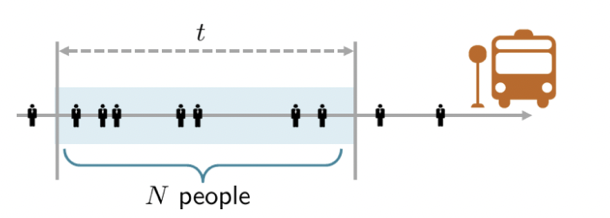
\includegraphics[scale=0.5]{img/poissonexpo1.png}
    \end{column}    
     \begin{column}{0.5\linewidth}
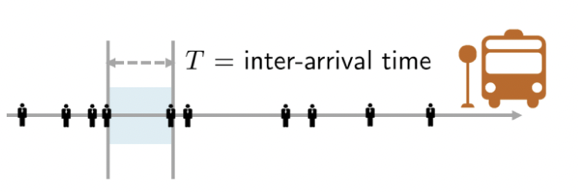
\includegraphics[scale=0.5]{img/poissonexpo2.png}
    \end{column} 
      \end{columns}
\end{frame}

\begin{frame}{\color{rosee}Variable aleatoria exponencial: pérdida de memoria}\small
  \begin{block}{}
    Otro uso de las variables exponenciales es para modelar el tiempo de
    vida de partes de un sistema, por ejemplo, el tiempo hasta que se
    quema una lamparita. Esto se debe en parte a que la distribución exponencial tiene la propiedad de falta de memoria.
  \end{block}
  \begin{proposition}[P\'erdida de memoria]
    Sea $X\sim Exp(\lambda)$. Entonces, si $t, t_0 >0$
    \[P\left( X \geq t+ t_{0}\mid X\geq t_{0}\right) =P\left( X \geq
      t\right) = e^{-\lambda t}.\]
  \end{proposition}
  \begin{alertblock}{Idea}
    Si ya sabemos que la lamparita dur\'o $t_0$ d\'ias, la probabilidad
    de que dure al menos $t$ d\'ias m\'as es igual a la probabilidad
    (no condicionada) de que la lamparita dure al menos $t$ d\'ias. El
    tiempo que le queda de funcionamiento a la lamparita es
    independiente de cuando tiempo de uso lleva.
  \end{alertblock}
\end{frame}

\begin{frame}{\color{rosee}Variable aleatoria exponencial: pérdida de memoria}\small
  \begin{proof}
    Si $t>0$
    \[P\left( X \leq t\right) = \int_{0}^{t} \lambda e^{-\lambda x}
    \, dx=-e^{-\lambda x} \vert_{0}^{t}= 1 - e^{-\lambda t}\,.\] Luego,
    \[P\left( X \geq t\right) = 1 - P\left( X < t\right) = 1 - \left(1 -
    e^{-\lambda t}\right) = e^{-\lambda t}.\] Entonces,
    \begin{align*}
      P\left( X \geq t+ t_{0}\mid X\geq
      t_{0}\right)&=\frac{P\left(\{ X \geq t+ t_{0} \}\cap
        \{ X\geq t_{0} \}\right)}{P\left(X\geq t_0 \right)}\\
      &= \frac{P\left(\{ X \geq t+ t_{0}
      \}\right)}{P\left(X\geq t_0 \right)}
      =\frac{e^{-\lambda(t+t_0)}}{e^{-\lambda t_0}}=e^{-\lambda t}.
    \end{align*}
  \end{proof}
\end{frame}

\begin{frame}{\color{rosee}Método de momentos: ejercicio 6}\small
  \begin{exampleblock}{Estimador de momentos para $\lambda$ si $X_i\stackrel{iid}{\sim} Exp(\lambda)$}
    Supongamos que el tiempo, \textbf{en minutos}, que pasa entre que llegan
    pedidos a un centro de distribuci\'on de una compa\~n\'ia
    alimenticia es una variable $X\sim Exp(\lambda)$.
    
    \begin{enumerate}
    \item Dada una muestra aleatoria $X_{1},\dots,X_{n}$,
      calcule el estimador de momentos de $\lambda$ usando el primer momento y muestre que es
      consistente para $\lambda$.
    \item Dada la siguiente muestra:
      \[ 2.63\quad 1.96\quad 0.13\quad 1.83\quad 0.44\quad 0.23\quad
      0.11\quad 0.06\quad 0.31\quad 0.44\]
      Obtenga el valor estimado para esta muestra. Para ese valor
      estimado, ¿c\'uanto estima que sea la probabilidad de que pase m\'as de un
      minuto entre dos pedidos?
      \item Ahora considere estimar a $\lambda$ usando el segundo momento. ¿Cómo cambia su respuesta? 
    \end{enumerate}
  \end{exampleblock}
\end{frame}


% \begin{frame}{\color{rosee}Variable aleatoria Pareto}
%   % Pablo: hacer Pareto o Rayleigh, mostrar que es consistente
%   \begin{definition}[Distribuci\'on Pareto]
%     Decimos que una variable aleatoria $X$ distribuci\'on
%     \textbf{pareto} con par\'ametros $\alpha$ y $\theta$ si su funci\'on
%     de densidad est\'a dada por
%     \[f_X(x|\alpha,\theta)=
%     \begin{cases}
%       \theta \alpha^{\theta} x^{-\theta-1} & \mbox{si} \; x\geq
%       \alpha.	 \\
%       0 & \mbox{en caso contrario}
%     \end{cases} \] donde $\alpha>0$ y $\theta>0$.
%   \end{definition}
%   \begin{block}{}
%     La distribuci\'on de Pareto es usada para modelar variables
%     aleatorias cuya densidad decae lentamente. Por ejemplo, en finanzas
%     se usa para modelar los retornos de acciones.
%   \end{block}
% \end{frame}

\begin{frame}{\color{rosee}M\'etodo de los momentos: pros y contras}
  \begin{block}{Ventajas}
    \begin{itemize}
    \item Es una idea intuitiva. Los estimadores son f\'aciles de calcular.
    \item Sirven estimar momentos poblacionales de modelos paramétricos y no paramétricos.
    \end{itemize}
  \end{block}
  \begin{block}{Desventajas}
    \begin{itemize}
    \item No est\'a guiado por ning\'un principio te\'orico (es
      ad-hoc).
      \item En el caso de la distribución exponencial vimos que, según el momento que se use para estimar al parámetro $\lambda$ la respuesta difiere. Es decir que es un método que puede dar dos estimadores distintos para el mismo parámetro en el mismo modelo poblacional.
    \item La teor\'ia asint\'otica (que veremos superficialmente)
      muestra que no en general no es \textbf{\'optimo}.
    \end{itemize}
    Por estas razones nos enfocaremos m\'as en el \textbf{m\'etodo de
      m\'axima verosimilitud} que estudiaremos con m\'as profundidad.
  \end{block}
\end{frame}

\begin{frame}{\color{rosee}Ejercicio Integrador}
Sea $X_1,\dots,X_n\stackrel{iid}{\sim}X$, donde $X\sim f(x;\theta) = \frac{1+x\theta}{2}$ si $x\in [-1,1]$ y con $\theta \in (-1,1)$.\bigskip
\begin{itemize}
    \item Halle el estimador de momentos de $\theta$ y verifique que es consistente e insesgado para $\theta$.\medskip
    \item Compute el ECM del estimador de momentos. ¿Qué ocurre con el ECM del estimador cuando $n\to \infty$?\medskip
    \item De una muestra de $n=10$ observaciones se tiene que $\sum_{i=1}^{10}x_i=0.7$; compute la estimación puntual usando el estimador de momentos de $\theta$ y estime el error estándar asociado a esta estimación.

\end{itemize}
\end{frame}

\end{document}


%%%
\begin{frame}{\color{rosee}Rao-Cr\'amer}
  La proposici\'on anteqrior nos dice que, en cierto sentido,
  $\overline{X}_{n}$ es `\'optimo' para estimar $E(X)$ si los datos son
  normales. Existe una maquinaria matem\'atica para \textbf{construir}
  estimadores IMV para problemas de estimaci\'on en general, pero queda
  afuera del alcance de este curso.

  \bigskip Lo que si veremos es que para una familia de problemas de
  estimaci\'on hay un l\'imite natural a la varianza que puede tener un
  estimador insesgado, dada por la cota de \textbf{Rao-Cramer}. Una vez
  probada esta cota, el teorema anterior para la normal se puede probar
  f\'acilmente.  La cota de Rao-Cramer esta intimamente relacionada con
  la funci\'on de verosimilitud, que a su vez est\'a relacionada con la
  noci\'on de \textbf{modelo param\'etrico}.
\end{frame}

\begin{frame}{\color{rosee}La funci\'on de verosimilitud}
  \begin{alertblock}{Notaci\'on}
    Usaremos la palabra densidad para referirnos tanto a la densidad de
    variables/vectores aleatorios continuos como a la funci\'on de
    probabilidad puntual de variables/vectores aleatorios discretos.
  \end{alertblock}
\end{frame}


\begin{frame}{\color{rosee}Modelos param\'etricos}
  C\'omo anticipamos, a continuaci\'on veremos que, para ciertos modelos
  param\'etricos, hay un l\'imite natural a que tan eficiente (poco
  variable) puede ser un estimador insesgado.
\end{frame}

\begin{frame}{\color{rosee}La funci\'on de verosimilitud}
  Supongamos que tenemos una muestra aleatoria $X_{1},\dots,X_{n}$.  El
  vector aleatorio $(X_{1},\dots,X_{n})$ tiene cierta funci\'on de
  densidad conjunta.

  \medskip Supongamos que esta funci\'on depende de un $\theta$
  (posiblemente un vector) desconocido. Digamos que
  $f(x_{1},\dots,x_{n};\theta)$ es la funci\'on de densidad de
  $(X_{1},\dots,X_{n})$ y que conocemos $f$, excepto por $\theta$.  Es
  decir, tenemos un modelo param\'etrico para la distribuci\'on de los
  datos.
\end{frame}

\begin{frame}{\color{rosee}La funci\'on de verosimilitud}
  Para cada $\theta$ fijo, mirando a $f(x_{1},\dots,x_{n};\theta)$ como
  funci\'on de $x_{1},\dots,x_{n}$, tenemos una funci\'on de
  densidad. Si dejamos $(x_{1},\dots,x_{n})$ fijo, y miramos a
  $f(x_{1},\dots,x_{n};\theta)$ como funci\'on de $\theta$, obtenemos la
  \textbf{funci\'on de verosimilitud}.

  \begin{definition}[Funci\'on de verosimilitud]
    Sea $f(x_{1},\dots,x_{n};\theta)$ la funci\'on de densidad de una
    muestra aleatoria $X_{1},\dots,X_{n}$, que depende de un par\'ametro
    desconocido $\theta$. La funci\'on
    \[L_{n}(\theta)=f(x_{1},\dots,x_{n};\theta),\]
    pensada c\'omo funci\'on de $\theta$ para $x_{1},\dots,x_{n}$ fijos,
    se llama la funci\'on de verosimilitud.
  \end{definition}
\end{frame}

\begin{frame}{\color{rosee}La funci\'on de verosimilitud} \small
  \begin{proposition}
    Sea $L_{n}(\theta)$ la funci\'on de verosimilitud de una muestra
    aleatoria $X_{1},\dots,X_{n}$. Llamemos $f(x;\theta)$ a la funci\'on
    de densidad que tienen en com\'un las v.a. de la muestra. Entonces
    \[L_{n}(\theta)= f(x_{1},\theta)f(x_{2},\theta)\dots f(x_{n},\theta)\]
  \end{proposition}
  \begin{proof}
    Como $X_{1},\dots,X_{n}$ son independientes, su funci\'on de
    densidad de factoriza. Luego
    \[L_{n}(\theta)=f(x_{1},\dots,x_{n};\theta)=
    f(x_{1},\theta)f(x_{2},\theta)\dots f(x_{n},\theta).\]
  \end{proof}
\end{frame}

\begin{frame}{\color{rosee}La funci\'on de verosimilitud} \small
  \begin{example}
    Sea $X_{1},\dots, X_{n}$ una muestra aleatoria de una normal con
    varianza conocida $\sigma^{2}=1$. El \'unico par\'ametro desconocido
    es entonces $\mu$, que jugar\'ia el rol de $\theta$ en la
    definici\'on anterior. La funci\'on de verosimilitud esta dada por
    \begin{align*}
      L_{n}(\theta) 
      &= \frac{1}{\sqrt{2\pi}}e^{\left(\frac{-(x_{1}-\theta)^{2}}{2} \right)}
        \dots \frac{1}{\sqrt{2\pi}}e^{\left(\frac{-(x_{n}-\theta)^{2}}{2} \right)}\\
      & = \left(\frac{1}{\sqrt{2\pi}}\right)^{n} e^{\left(\frac{-\sum_{i=1}^{n}
        (x_{i}-\theta)^{2}}{2}\right)}
    \end{align*}
  \end{example}
\end{frame}

\begin{frame}{\color{rosee}La funci\'on de verosimilitud}\small
  \begin{exampleblock}{Ejemplo}
    Sea $X_{1},\dots, X_{n}$ una muestra aleatoria de una normal. En
    este caso no conocemos $\sigma$, as\'i que $\theta=(\mu,
    \sigma)$. La verosimilitud es
    \begin{align*}
      L_{n}(\theta)
      &= \frac{1}{\sqrt{2\pi\sigma^{2}}}e^{\left(\frac{-(x_{1}-\mu)^{2}}{2\sigma^{2}}
        \right)}\dots \frac{1}{\sqrt{2\pi\sigma^{2}}}
        e^{\left(\frac{-(x_{n}-\mu)^{2}}{2\sigma^{2}} \right)}\\
      & = \left(\frac{1}{\sqrt{2\pi\sigma^{2}}}\right)^{n} 
        e^{\left(\frac{-\sum_{i=1}^{n} (x_{i}-\mu)^{2}}{2\sigma^{2}}\right)}
    \end{align*}
  \end{exampleblock}
\end{frame}

\begin{frame}{\color{rosee}La funci\'on de verosimilitud}\small
  \begin{exampleblock}{Ejemplo}
    Sea $X_{1},\dots, X_{n}$ una muestra aleatoria de una Ber(p). En
    este caso, el par\'ametro $\theta$ es igual a $p$. La verosimilitud
    es
    \begin{align*}
      L_{n}(\theta) 
      &= p^{x_{1}} (1-)^{1-x_{1}}\dots p^{x_{n}} (1-)^{1-x_{n}}\\
      & = p^{\sum_{i=1}^{n}x_{i}} (1-p)^{n-\sum_{i=1}^{n}x_{i}}
    \end{align*}
  \end{exampleblock}
\end{frame}

\begin{frame}{\color{rosee}La funci\'on de verosimilitud}
  Por qu\'e el nombre `verosimilitud'? Veamos el ejemplo de la
  Bernoulli. Supongamos que $n=4$, $x_{1}=0, x_{2}=1, x_{3}=0$ y
  $x_{4}=0$. Entonces
  \[l_{4}(1/3)= \frac{1}{3}\left(\frac{2}{3}\right)^{3} \approx 0.14\]
  \[l_{4}(3/4)=\frac{3}{4} \left(\frac{1}{4}\right)^{3} \approx 0.01\]
  Es m\'as probable haber obtenido la muestra que tenemos si $p$ fuera
  $1/3$ que si $p$ fuera $3/4$.

  \medskip Esto nos da una idea para estimar, elegir el $\theta$ que
  maximice la verosimilitud. Esta es la idea detr\'as del m\'etodo de
  m\'axima verosimilitud, que veremos m\'as adelante.
\end{frame}

\begin{frame}{\color{rosee}El score}
  A partir de ahora supondremos que $\theta\in \mathbb{R}$.

  \begin{definition}[Score]
    La funci\'on de score de $\theta$, para el caso de $\theta$ un
    n\'umero real est\'a dada por
    \[s_{n}(\theta)=
    \frac{d\log(L_{n}(\theta))}{d\theta}=\frac{d\log(f(x_{1},\dots,x_{n};
      \theta)}{d\theta}.\]
    % Si $\theta=(\theta_{1},\dots,\theta_{r})$ es un vector de $r$ coordenadas
    % \begin{align*}
    %   s(\theta)&= \nabla \log(f(x_{1},\dots,x_{n}; \theta)
    %   \\
    %   &=\left(\frac{d\log(f(x_{1},\dots,x_{n}; \theta)}{d\theta_{1}},\dots,\frac{d\log(f(x_{1},\dots,x_{n}; \theta)}{d\theta_{r}} \right).
    % \end{align*}
    \textbf{El score es una funci\'on \'unicamente de $\theta$.}
  \end{definition}
\end{frame}

\begin{frame}{\color{rosee}El score}
  \begin{definition}[Score (aleatorio)]
    Consideremos ahora para el caso de $\theta$ un n\'umero real
    \[S_{n}(\theta)= \frac{d\log(f(X_{1},\dots,X_{n}; \theta)}{d\theta}.\]
    % y si $\theta=(\theta_{1},\dots,\theta_{r})$ es un vector de $r$ coordenadas
    % \begin{align*}
    %   S(\theta)&= \nabla \log(f(X_{1},\dots,X_{n}; \theta).
    % \end{align*}
  \end{definition}
  \begin{alertblock}{Ojo}
    La diferencia entre $s_{n}(\theta)$ y $S_{n}(\theta)$ es que
    $S_{n}(\theta)$ es una variable aleatoria. Lamentablemente, por
    razones hist\'oricas, a ambas se las conoce con el nombre de
    score. Para tratar de evitar la confusion a $S_{n}(\theta)$ la
    llamaremos el score aleatorio.
  \end{alertblock}
\end{frame}

\begin{frame}{\color{rosee}El score}
  \begin{proposition}
    Bajo \textbf{condiciones de regularidad}
    \[E_{\theta}(S_{n}(\theta))=0,\]
    donde $E_{\theta}(\cdot)$ quiere decir que la esperanza se calcula
    usando $\theta$ como valor verdadero del par\'ametro.
  \end{proposition}
\end{frame}

\begin{frame}{\color{rosee}El score}
  \begin{proof}
    Lo hacemos para el caso de continuas.
    \begin{align*}
      E_{\theta}(S_{n}(\theta)) &= \int \frac{d\log(f(x_{1},\dots,x_{n}; \theta)}{d\theta} f(x_{1},\dots,x_{n};\theta) dx_{1}\dots dx_{n}
      \\&
          =\int \frac{\frac{d f(x_{1},\dots,x_{n}; \theta}{d\theta}}{f(x_{1},\dots,x_{n};\theta)} f(x_{1},\dots,x_{n};\theta) dx_{1}\dots dx_{n}
      \\&
          =\int \frac{d f(x_{1},\dots,x_{n}; \theta)}{d\theta}dx_{1}\dots dx_{n}
      \\&
          \underbrace{=}_{\text{delicado}} \frac{d}{d\theta} \int f(x_{1},\dots,x_{n}; \theta) dx_{1}\dots dx_{n}= \frac{d}{d\theta} 1 = 0.
    \end{align*}
  \end{proof}
\end{frame}

\begin{frame}{\color{rosee}El score}

  \begin{proposition}
    Bajo \textbf{condiciones de regularidad}
    $$
    Var_{\theta}(S_{n}(\theta))=E_{\theta}(S_{n}^{2}(\theta))= -E_{\theta}\left( \frac{d}{d\theta} S_{n}(\theta) \right) ,
    $$
    donde $Var_{\theta}(\cdot)$ quiere decir que la esperanza se calcula usando $\theta$ como valor verdadero del par\'ametro.
  \end{proposition}


\end{frame}

\begin{frame}{\color{rosee}El score}
  \begin{proof}
    La primer igualdad es inmediata por la proposici\'on anterior. Ahora, vimos que
    \begin{align*}
      0= \int s_{n}(\theta) f(x_{1},\dots,x_{n}; \theta) dx_{1}\dots dx_{n}.
    \end{align*}
    Derivando de ambos lados de la igualdad y metiendo la derivada adentro de la integral (esto es lo delicado...)
    \begin{align*}
      0&= \int \frac{d}{d\theta} (s_{n}(\theta) f(x_{1},\dots,x_{n}; \theta)) dx_{1}\dots dx_{n}
      \\&
          = \int \frac{d}{d\theta} s_{n}(\theta) f(x_{1},\dots,x_{n}; \theta) dx_{1}\dots dx_{n} +
      \\& \int  s_{n}(\theta) \frac{d}{d\theta}f(x_{1},\dots,x_{n}; \theta) dx_{1}\dots dx_{n}.
    \end{align*}
  \end{proof}

\end{frame}

\begin{frame}{\color{rosee}El score}
  \begin{proof}
    \small
    Luego 
    \begin{align*}
      -E_{\theta}\left(\frac{d}{d\theta} S_{n}(\theta)\right)&=-\int \frac{d}{d\theta} s_{n}(\theta) f(x_{1},\dots,x_{n}; \theta) dx_{1}\dots dx_{n} 
      \\& 
          =\int  s_{n}(\theta) \frac{d}{d\theta}f(x_{1},\dots,x_{n}; \theta) dx_{1}\dots dx_{n}.
    \end{align*}
    Pero 
    \begin{align*}
      &\int  s_{n}(\theta) \frac{d}{d\theta}f(x_{1},\dots,x_{n}; \theta) dx_{1}\dots dx_{n} =
      \\& \int  \frac{\frac{d f(x_{1},\dots,x_{n}; \theta}{d\theta}}{f(x_{1},\dots,x_{n};\theta)} \frac{d}{d\theta}f(x_{1},\dots,x_{n}; \theta) dx_{1}\dots dx_{n}=
      \\& \int  \left(\frac{\frac{d f(x_{1},\dots,x_{n}; \theta}{d\theta}}{f(x_{1},\dots,x_{n};\theta)}\right)^{2} f(x_{1},\dots,x_{n}; \theta) dx_{1}\dots dx_{n}=E_{\theta}(S_{n}(\theta)^{2}).
    \end{align*}
  \end{proof}

\end{frame}

\begin{frame}{\color{rosee}Informaci\'on de Fisher}
  \begin{definition}[Informaci\'on de Fisher]
    La informaci\'on de Fisher, denotada $I_{n}(\theta)$, se define como
    $$
    I_{n}(\theta)=E_{\theta}\left( S_{n}^{2}(\theta) \right).
    $$
  \end{definition}
  \begin{alertblock}{Idea}
    La informaci\'on de Fisher nos dice cuanta informaci\'on hay en una muestra de tama\~no $n$ sobre el par\'ametro $\theta$.
  \end{alertblock}

\end{frame}

\begin{frame}{\color{rosee}Informaci\'on de Fisher}
  \begin{proposition}
    $$
    I_{n}(\theta)=n I_{1}(\theta).
    $$
  \end{proposition}
  \begin{alertblock}{Idea}
    La informaci\'on crece linealmente con el n\'umero de observaciones.
  \end{alertblock}

\end{frame}

\begin{frame}{\color{rosee}Informaci\'on de Fisher}
  \small
  \begin{proof}
    \begin{align*}
      &I_{n}(\theta)= E_{\theta}\left( S_{n}^{2}(\theta) \right) = Var_{\theta}\left( S_{n}(\theta) \right)= Var_{\theta}\left( \frac{d}{d\theta} \log(f(x_{1};\theta)\dots f(x_{n};\theta)) \right)=
      \\&
          Var_{\theta}\left( \frac{d}{d\theta} \sum_{i=1}^{n}\log(f(x_{i};\theta)) \right)=Var_{\theta}\left(  \sum_{i=1}^{n} \frac{d}{d\theta}\log(f(x_{i};\theta)) \right)=
      \\&
          \sum\limits_{i=1}^{n} Var_{\theta}\left( \frac{d}{d\theta}\log(f(x_{i};\theta))\right)=\sum\limits_{i=1}^{n} I_{1}(\theta)= nI_{1}(\theta).
    \end{align*}
  \end{proof}
  \begin{alertblock}{}
    Notar que usamos fuertemente que $X_{1},\dots, X_{n}$ son i.i.d.
  \end{alertblock}
\end{frame}

\begin{frame}{\color{rosee}Informaci\'on de Fisher}
  \small
  \begin{example}[Poisson]
    Supongamos que $X_{1},\dots, X_{n}$ son Pois($\lambda$). Entonces $\theta=\lambda$. La verosimilitud es
    $$
    L_{n}(\theta)=e^{-\theta} \frac{\theta^{x_{1}}}{x_{1}!}\dots e^{-\theta} \frac{\theta^{x_{n}}}{x_{n}!} = \frac{\exp(-n\theta) \theta^{\sum_{i=1}^{n} x_{i}}}{\prod_{i=1}^{n} x_{i}!}.
    $$
    $$
    \log(L_{n}(\theta))= -n\theta + \sum_{i=1}^{n}x_{i} \log(\theta) + \log(\prod_{i=1}^{n} x_{i}!).
    $$
    $$
    \frac{d}{d\theta}\log(L_{n}(\theta))= -n+ \sum_{i=1}^{n}x_{i} \frac{1}{\theta}.
    $$
    $$
    \frac{d^{2}}{d\theta^{2}}\log(L_{n}(\theta))= -\sum_{i=1}^{n}x_{i} \frac{1}{\theta^{2}}.
    $$
    $$
    I_{n}(\theta)= -E\left(-\sum_{i=1}^{n}X_{i} \frac{1}{\theta^{2}}\right) =\frac{1}{\theta^{2}} \sum_{i=1}^{n}E(X_{i}) = \frac{n}{\theta}.  
    $$
  \end{example}
\end{frame}


\begin{frame}{\color{rosee}Informaci\'on de Fisher}
  \small
  \begin{example}[Bernoulli]
    Supongamos que $X_{1},\dots, X_{n}$ son Ber($p$). Entonces $\theta=p$. La verosimilitud es
    $$
    L_{n}(\theta)=\theta^{\sum_{i=1}^{n} x_{i}} (1-\theta)^{(n-{\sum_{i=1}^{n} x_{i}})}.
    $$
    $$
    \log(L_{n}(\theta))= (\sum_{i=1}^{n} x_{i}) \log(\theta)+ (n-\sum_{i=1}^{n} x_{i}) \log(1-\theta).
    $$
    $$
    \frac{d}{d\theta}\log(L_{n}(\theta))=(\sum_{i=1}^{n} x_{i}) \frac{1}{\theta}- (n-\sum_{i=1}^{n} x_{i}) \frac{1}{1-\theta}.
    $$
    $$
    \frac{d^{2}}{d\theta^{2}}\log(L_{n}(\theta))= -(\sum_{i=1}^{n} x_{i}) \frac{1}{\theta^{2}}- (n-\sum_{i=1}^{n} x_{i}) \frac{1}{(1-\theta)^{2}}.
    $$
    $$
    I_{n}(\theta)= -E\left(-(\sum_{i=1}^{n} x_{i}) \frac{1}{\theta^{2}}- (n-\sum_{i=1}^{n} x_{i}) \frac{1}{(1-\theta)^{2}}\right)  = \frac{n}{\theta (1-\theta)}.  
    $$
  \end{example}
\end{frame}


\begin{frame}{\color{rosee}Cota de Rao-Cramer}
  \begin{theorem}
    Sea $\widehat{\theta}_{n}$ un estimador insesgado de $\theta$. Entonces \textbf{bajo condiciones de regularidad}
    $$ 
    Var(\widehat{\theta}_{n})\geq \frac{1}{I_{n}(\theta)} = \frac{1}{n I_{1}(\theta)}.
    $$
  \end{theorem}

  \begin{alertblock}{Idea}
    La m\'inima varianza que puede tener un estimador insesgado de $\theta$ es $\frac{1}{n I_{1}(\theta)}$. Si un estimador tiene esta varianza, es decir, si alcanza la cota, tiene que ser el IMV. En este caso, decimos que el estimador es eficiente.
  \end{alertblock}
\end{frame}

\begin{frame}{\color{rosee}Cota de Rao-Cramer}
  \small
  \begin{proof}
    La hacemos para el caso de continuas. Como $\widehat{\theta}_{n}$ es insesgado
    \begin{align*}
      \theta= E_{\theta}(\widehat{\theta}_{n})= \int \widehat{\theta}_{n}(x_{1},\dots,x_{n}) f(x_{1},\dots,x_{n};\theta)dx_{1}\dots dx_{n}.
    \end{align*}
    Tomando derivadas de ambos lados y metiendo la derivada dentro de la integral (delicado)
    \begin{align*}
      1&= \int \widehat{\theta}_{n}(x_{1},\dots,x_{n}) \frac{d}{d\theta}f(x_{1},\dots,x_{n};\theta)
      \\&
          =\int \widehat{\theta}_{n}(x_{1},\dots,x_{n}) \frac{\frac{d}{d\theta}f(x_{1},\dots,x_{n};\theta)}{f(x_{1},\dots,x_{n};\theta)}f(x_{1},\dots,x_{n};\theta) dx_{1}\dots dx_{n}
      \\&
          =\int \widehat{\theta}_{n}(x_{1},\dots,x_{n}) s_{n}(\theta)f(x_{1},\dots,x_{n};\theta) dx_{1}\dots dx_{n}
      \\&
          = E_{\theta} \left( \widehat{\theta}_{n} S_{n}(\theta) \right).
    \end{align*}
  \end{proof}
\end{frame}

\begin{frame}{\color{rosee}Cota de Rao-Cramer}
  \small
  \begin{proof}
    Como $E_{\theta}(S_{n})=0$, tenemos que $cov(S_{n}(\theta), \widehat{\theta}_{n})=1$.
    Por otro lado
    $$
    corr(S_{n}(\theta), \widehat{\theta}_{n}) = \frac{cov(S_{n}(\theta), \widehat{\theta}_{n})}{\sqrt{Var( S_{n}(\theta))Var(\widehat{\theta}_{n}) }}= \frac{1}{\sqrt{Var( S_{n}(\theta))Var(\widehat{\theta}_{n}) }}\leq 1.
    $$
    Luego
    $$
    Var(\widehat{\theta}_{n})  \geq \frac{1}{Var( S_{n}(\theta))}=\frac{1}{I_{n}(\theta)}.
    $$
  \end{proof}
\end{frame}

\begin{frame}
  \begin{example}[Poisson, $\theta=\lambda$]
    La cota de Rao-Cramer es 
    $$
    \frac{1}{n/\theta}=\frac{\theta}{n}.
    $$
    $\overline{X}_{n}$ es insesgado para $\theta$ y 
    $$
    Var(\overline{X}_{n})=\frac{\theta}{n}.
    $$
    Por lo tanto $\overline{X}_{n}$ alcanza la cota de Rao-Cramer y es el IMV para $\theta$.
  \end{example}

\end{frame}

\begin{frame}
  \begin{example}[Bernoulli, $\theta=p$]
    La cota de Rao-Cramer es 
    $$
    \frac{1}{n/(\theta (1-\theta))}=\frac{\theta(1-\theta)}{n}.
    $$
    $\overline{X}_{n}$ es insesgado para $\theta$ y 
    $$
    Var(\overline{X}_{n})=\frac{\theta(1-\theta)}{n}.
    $$
    Por lo tanto $\overline{X}_{n}$ alcanza la cota de Rao-Cramer y es el IMV para $\theta$.
  \end{example}
\end{frame}

\begin{frame}
  \begin{alertblock}{Ejercicio}
    Supongamos que $X_{1},\dots, X_{n}$ son normales con varianza igual
    a 1 y media $\mu$. Mostrar que $\overline{X}_{n}$ es el IMV para
    $\mu$.
  \end{alertblock}
\end{frame}

\begin{frame}
  Pablo: escribite algo sobre el caso multivariado, todo atado con
  alambre, ponele que solo en dos dimensiones, por ejemplo la normal con
  mu y sigma
\end{frame}

%https://tex.stackexchange.com/questions/164991/pgfplots-how-to-fill-bounded-area-under-a-curve-using-addplot-and-fill

%https://tex.stackexchange.com/questions/140312/tikz-shading-region-bounded-by-several-curves
%tikz para graficar areas

%http://latexcolor.com/

%https://www.tablesgenerator.com/
\PassOptionsToPackage{force}{filehook}

\documentclass{beamer}


\usepackage[utf8]{inputenc}
\usepackage{amsmath}
\usepackage{amssymb}% http://ctan.org/pkg/amssymb
\usepackage{amsfonts}
\usepackage{pifont}% http://ctan.org/pkg/pifont
%https://tex.stackexchange.com/questions/42619/x-mark-to-match-checkmark
\newcommand{\cmark}{\ding{51}}
\newcommand{\xmark}{\ding{55}}
%\usepackage{amsfonts}
\usepackage{graphicx} 
\usepackage{subcaption}
\usepackage{hyperref}
\usepackage{cancel}
\usepackage{wrapfig}
\usepackage{enumitem}
\usepackage{comment}
\hypersetup{
	colorlinks=true,
	linkcolor=blue,
	filecolor=magenta,      
	urlcolor=cyan,
}
\newtheorem*{proposicion}{Proposici\'on}
\newtheorem*{teorema}{Teorema}
\renewcommand*{\proofname}{Demostraci\'on}
\newtheorem*{ejercicio}{Ejercicio}
\usepackage{pgf,tikz}
\usetikzlibrary{positioning}
\usetikzlibrary{arrows,patterns}
\usetikzlibrary{arrows.meta}
\usepackage[spanish, activeacute]{babel} %Definir idioma español
\usepackage[utf8]{inputenc} %Codificacion utf-8
\usepackage{multirow}

%   Esconder las soluciones
\newif\ifhideproofs
\hideproofstrue %uncomment to hide proofs

\ifhideproofs
\usepackage{environ}
\NewEnviron{hide}{}
\let\solucion\hide
\let\endsolucion\endhide
\fi

\usepackage{color}
\usepackage{mathpazo}
\usepackage{hyperref}
\usepackage{multimedia}
\usepackage{graphicx}
\usepackage{textcomp}
\usepackage[spanish, activeacute]{babel} 
\usepackage{graphicx} 
\usepackage{booktabs}
\usepackage{cite}
\usepackage{hyperref}
\usepackage{multicol}
\usepackage{multirow,array}

\usepackage{mathrsfs}
%\usepackage{amssymb}

\usepackage{tabularx}
    \newcolumntype{L}{>{\raggedright\arraybackslash}X}
        %\newcolumntype{b}{>{\hsize=1.5\hsize}X}
    %\newcolumntype{s}{>{\hsize=.9\hsize}X}

\usepackage{amsthm}
\newtheorem{thm}{Teorema}
\newtheorem{lem}[thm]{Lema}
\newtheorem{axiom}[thm]{Axioma}
\newtheorem{prop}[thm]{Proposici\'on}
\newtheorem{coro}[thm]{Corolario}
\theoremstyle{definition}
\newtheorem{defn}{Definici\'on}
\DeclareGraphicsExtensions{.pdf,.jpeg,.png,.eps}
\usetheme{CambridgeUS}
\setbeamertemplate{navigation symbols}{}

%Paréntisis y otros
\newcommand{\cmc}{\overset{m.c.}{\rightarrow}}
\newcommand{\p}[1]{\left(#1\right)}
\newcommand{\cor}[1]{\left[#1\right]}
\newcommand{\lla}[1]{\left\{#1\right\}}
\newcommand{\eps}{\varepsilon}
\newcommand{\lol}{\mathcal{L}}
\newcommand{\RR}{\mathbb{R}}
\newcommand{\QQ}{\mathbb{Q}}
\newcommand{\NN}{\mathbb{N}}
\newcommand{\paren}[1]{\left(#1\right)}
\newcommand{\corc}[1]{\left[#1\right]}
\newcommand{\llav}[1]{\left\lbrace#1\right\rbrace}
\newcommand{\partt}[1]{\left(\text{#1}\right)}
\newcommand{\corctt}[1]{\left[\text{#1}\right]}
\newcommand{\llavtt}[1]{\left\lbrace\text{#1}\right\rbrace}
\makeatletter
\def\munderbar#1{\underline{\sbox\tw@{$#1$}\dp\tw@\z@\box\tw@}}
\makeatother

%\usepackage[scr=rsfs,cal=boondox]{mathalfa}
\usepackage[scr=esstix,cal=boondox]{mathalfa}

% \usepackage{mdframed}
% \newmdtheoremenv{solucion}{Soluci\'on}

% Enmarcar las soluciones
% \newenvironment{solu}
% {%
% \begin{framed}
%   \begin{solucion}
%   }%
%     {%     
%   \end{solucion}
% \end{framed}
% }

%   Esconder las soluciones
\newif\ifhideproofs
%\hideproofstrue %uncomment to hide proofs

\ifhideproofs
\usepackage{environ}
\NewEnviron{hide}{}
\let\solucion\hide
\let\endsolucion\endhide
\fi



%Graficos y cosas
\usepackage{amssymb}
\usepackage{tikz}
\usepackage{pgfplots}
\usepackage{mathtools}
\usepackage{xcolor}
%\pgfplotsset{compat=1.9}
\usepgfplotslibrary{fillbetween,decorations.softclip}
\pgfplotsset{compat = newest}
\usepackage{pst-func}
\usepackage{pstricks}
\usepackage{pst-plot}

% Comando para usar multiples footnotes en un align environment

\makeatletter
\newcommand{\AlignFootnote}[1]{%
    \ifmeasuring@
    \else
        \footnote{#1}%
    \fi
}
\makeatother

%https://tex.stackexchange.com/questions/82782/footnote-in-align-environment


\DeclareGraphicsExtensions{.pdf,.jpeg,.png,.eps}
\usepackage{tikz}
%\usepackage{tikz-cd}
\usetikzlibrary{decorations}
%\usetikzlibrary{snakes}
\usetikzlibrary{cd}

\useoutertheme{split}
\useinnertheme{rounded}


%\beamertemplatenavigationsymbolsempty  %removes navigation bar
\definecolor{rosee}{rgb}{0.7,0.05,0.25}
\definecolor{pacificorange}{cmyk}{0,.6,1,0} %approved Pacific colors 2010
\definecolor{pacificgray}{cmyk}{0,.15,.35,.60}
\definecolor{pacificlgray}{cmyk}{0,0,.2,.4}
\definecolor{pacificcream}{cmyk}{.05,.05,.15,0}
\definecolor{deepyellow}{cmyk}{0,.17,.80,0}
\definecolor{lightblue}{cmyk}{.49,.01,0,0}
\definecolor{lightbrown}{cmyk}{.09,.15,.34,0}
\definecolor{deepviolet}{cmyk}{.79,1,0,.15}
\definecolor{deeporange}{cmyk}{0,.59,1,18}
\definecolor{dustyred}{cmyk}{0,.7,.45,.4}
\definecolor{grassgreen}{RGB}{92,135,39}
\definecolor{pacificblue}{RGB}{59,110,143}
\definecolor{pacificgreen}{cmyk}{.15,0,.45,.30}
\definecolor{deepblue}{cmyk}{1,.57,0,2}
\definecolor{turquoise}{cmyk}{.43,0,.24,0}
\definecolor{gren}{rgb}{0.2,0.8,0.5}
\definecolor{orang}{rgb}{1,0.64,0}
\definecolor{amethyst}{rgb}{0.6, 0.4, 0.8}
\definecolor{dodgerblue}{rgb}{0.12, 0.56, 1.0}
\definecolor{fandango}{rgb}{0.71, 0.2, 0.54}
\definecolor{forestgreen(traditional)}{rgb}{0.0, 0.27, 0.13}
\definecolor{iris}{rgb}{0.35, 0.31, 0.81}
\definecolor{jazzberryjam}{rgb}{0.65, 0.04, 0.37}
\definecolor{mediumjunglegreen}{rgb}{0.11, 0.21, 0.18}
\definecolor{mediumpersianblue}{rgb}{0.0, 0.4, 0.65}
\definecolor{midnightgreen}{rgb}{0.0, 0.29, 0.33}
\definecolor{orangee}{rgb}{1.0, 0.5, 0.0}

% There are many different themes available for Beamer. A comprehensive
% list with examples is given here:
% http://deic.uab.es/~iblanes/beamer_gallery/index_by_theme.html
% You can uncomment the themes below if you would like to use a different
% one:
%\usetheme{AnnArbor} %boca
%\usetheme{Antibes} %azul y gris
%\usetheme{Bergen} %barra who where
%\usetheme{Berkeley} %bordes
%usetheme{Berlin} %blanco y azul
%\usetheme{Boadilla}
%\usetheme{boxes}
\usetheme{CambridgeUS}
%\usetheme{Copenhagen}
%\usetheme{Darmstadt}
%\usetheme{default}
%\usetheme{Frankfurt}
%\usetheme{Goettingen}
%\usetheme{Hannover}
%\usetheme{Luebeck}
%\usetheme{Malmoe}
%\usetheme{Marburg}
%\usetheme{Montpellier}
%\usetheme{PaloAlto}
%\usetheme{Pittsburgh}
%\usetheme{Rochester}
%\usetheme{Singapore}
%\usetheme{Szeged}
%\usetheme{Warsaw}

%\usecolortheme{beaver}
%\usecolortheme{whale}
%\usecolortheme{orchid}
%\usecolortheme{wolverine}
%\usecolortheme[named=pacificblue]{structure} %replaces the blue of Copenhagen with Pacific orange

\definecolor{myNewColorA}{rgb}{0,0,100}
\definecolor{myNewColorB}{rgb}{0,100,100}
\definecolor{myNewColorC}{rgb}{0,200,100}
\definecolor{myNewColorD}{rgb}{0,100,200}

%\setbeamercolor*{palette primary}{bg=myNewColorA, fg = black}
%\setbeamercolor*{palette secondary}{bg=myNewColorB, fg = black}
%\setbeamercolor*{palette tertiary}{bg=myNewColorC, fg = black}
%\setbeamercolor*{palette quaternary}{bg=myNewColorD, fg = black}

\setbeamercolor*{palette primary}{bg=rosee, fg = white}
\setbeamercolor*{palette secondary}{bg=gren, fg = white}
\setbeamercolor*{palette tertiary}{bg=-red!75!, fg = white}
\setbeamercolor*{palette quaternary}{bg=-red!75!, fg = white}

\newtheorem{proposition}{Proposici\'on}
\newcommand{\ton}{\underset{n\to\infty}{\longrightarrow}}
\newcommand{\cp}{\overset{P}{\rightarrow}}
\newcommand{\cw}{\overset{d}{\rightarrow}}

%\expandafter\def\expandafter\insertshorttitle\expandafter{%
 % \insertshorttitle\hfill%
  %\insertframenumber\,/\,\inserttotalframenumber}

%\mode
%<all>

%Para agrandar el espacio entre renglones de las tablas
%https://tex.stackexchange.com/questions/26690/how-to-add-extra-spaces-between-rows-in-tabular-environment
\renewcommand{\arraystretch}{1.5}

\usepackage{color, xcolor}
\definecolor{codegreen}{rgb}{0,0.6,0}
\definecolor{codegray}{rgb}{0.5,0.5,0.5}
\definecolor{codepurple}{rgb}{0.58,0,0.82}
\definecolor{backcolour}{rgb}{0.95,0.95,0.92}

\usepackage{listings}
\lstdefinestyle{mystyle}{
  backgroundcolor=\color{backcolour},   
  commentstyle=\color{codegreen},
  language = R,
  % commentchar=\#,
  keywordstyle=\color{magenta},
  numberstyle=\tiny\color{codegray},
  stringstyle=\color{codepurple},
  basicstyle=\ttfamily\footnotesize,
  breakatwhitespace=false,         
  breaklines=false,                 
  captionpos=b,                    
  frame=single,
  keepspaces=false,
  % numbers=left,                    
  % numbersep=pt,                  
  % columns=flexible,
  stepnumber=1,
  resetmargins=true,
  showspaces=false,                
  showstringspaces=false,
  showtabs=false,                  
  tabsize=1
}
\lstset{style=mystyle}
  



\def\mydate{\leavevmode\hbox{\twodigits\day/\twodigits\month/\the\year}}
\def\twodigits#1{\ifnum#1<10 0\fi\the#1}

\usepackage[final]{pdfpages}

% PARA AGREGAR IMAGEN EN EL FONDO DE LAS SLIDES
\usebackgroundtemplate%
%{%
 %
\includegraphics[width=\paperwidth,height=\pape%rheight]{slides1/fondo.png}%  
%}


\title{\color{black}{Análisis Estadístico}}
\subtitle{Estimación Puntual I \footnote{Basado en las notas de Ezequiel Smucler y Lara Sánchez Peña}}
\institute[]{UTDT}
\medskip
\date[UTDT 2021]{}

\begin{document}
\begin{frame}
  \titlepage
\end{frame}


\begin{frame}{\color{rosee}Estimaci\'on (refresh de conceptos)}
  \begin{block}{El 'Problema de Estimaci\'on'}
Dada $\textbf{X}\equiv \{X_{1}, \dots, X_{n}\}\stackrel{iid}{\sim} X$ queremos construír un estimador $\widehat{\theta}_{n}(\textbf{X})$ de algún parámetro $\theta$ asociado a la distribuci\'on de $X$ en la población. A cada realización de la muestra le corresponderá una estimación de $\theta$; si nuestro estimador tiene \textit{buenas propiedades} entonces esperamos (confiamos) que la estimación del parámetro que obtuvimos con los datos sea certera.
  \end{block}
\medskip
\begin{itemize}
    \item Ejemplo I: $\theta = E(X)$ y $\widehat{\theta}_{n}(\textbf{X}) = \overline{X}_n$\medskip
\item Ejemplo II: $\theta = Var(X)$ y $\widehat{\theta}_{n}(\textbf{X}) = \sum_{i=1}^n(X_i - \overline{X}_n)^2/n=\widehat{\sigma}^2$.\medskip
\item Ejemplo práctico en \texttt{R} o Excel.
\end{itemize}

%  \begin{definition}[Estimador]
%    Dadas variables aleatorias $X_{1},\dots,X_{n}$, para un par\'ametro
%    cualquiera $\theta$, un \textbf{estimador} es una funci\'on de
%    $X_{1},\dots,X_{n}$.
%  \end{definition}

  \begin{alertblock}{Algunos puntos a tener en cuenta:}
\begin{itemize}
    \item No confundir estimador con estimación.\medskip
    \item ¿Cómo \underline{medimos} la \textbf{calidad} de un estimador?
\end{itemize}
  \end{alertblock}
\end{frame}

\begin{frame}%{Estimaci\'on} \small 
  \begin{block}{}
    Ya discutimos una propiedad \textbf{asint\'otica} indispensable de un estimador: la \textbf{consistencia}. A continuaci\'on, estudiaremos
    algunas propiedades para \textbf{muestras finitas} (no
    asint\'oticas) para estudiar la calida de los mismos.
  \end{block}
  
  \begin{block}{Preguntas que vamos a responder:}
    \begin{itemize}
\medskip
    \item  ¿C\'omo medimos si un estimador es \textbf{mejor}
      que otro? \medskip
      \item ¿C\'ual es la manera \textbf{\'optima} de estimar un       par\'ametro?\medskip
      
\item En algunos contextos específicos podremos incluso determinar la  \textbf{distribuci\'on muestral} del estimador, y esto nos permite responder:\medskip
\begin{itemize}
    \item ¿Podemos garantizar que, con probabilidad alta, el estimador va a estar \textbf{cerca} del valor verdadero (y desconocido) del parámetro?\medskip
\item ¿Cu\'antas (y qu\'e tipo de) observaciones necesitamos para garantizar cierto margen de error con probabilidad alta?
\end{itemize}
    \end{itemize}
  \end{block}

\end{frame}

\begin{frame}{\color{rosee}Ejemplo motivacional (calidad de un estimador)} \small 
  \begin{exampleblock}{Estimar el par\'ametro de una Bernoulli}
Dada una muestra aleatoria $\{X_{1},\dots, X_{n}\} \sim \text{Bern}(p)$, llamemos
    \[T = \sum_{i=1}^{n}X_{i}\] Proponemos tres estimadores de $p=E(X)$:
    \begin{itemize}
    \item La media muestral: \[\widehat{p}_{1}= T/n = \overline{X}_{n}\,.\]
    \item La media muestral agregando $2$ fracasos y $2$ \'exitos
      ``artificiales'' a la muestra:
      \[\widehat{p}_{2} = \frac{T + 2}{n+4}\,.\]
    \item La media muestral de solo dos observaciones:
      \[\widehat{p}_{3} = \frac{X_{1}+X_{2}}{2}\,.\]
    \end{itemize}
  \end{exampleblock}
\end{frame}

\begin{frame}{\color{rosee}Ejemplo motivacional (calidad de un estimador)} \small
  \begin{exampleblock}{Estimar el par\'ametro de una Bernoulli}
    \begin{description}
    \item[$\widehat{p}_{1}$] sabemos que es consistente por LGN.
    \item[$\widehat{p}_{2}$] tambi\'en es consistente (¿por qu\'e?).\\~\\~\\~\\~\\
    \item[$\widehat{p}_{3}$] no es consistente (est\'a \textit{tirando} informaci\'on).\\~\\~\\~\\~\\
    \end{description}
    \end{exampleblock}
    \medskip
\begin{itemize}
    \item Descartamos $\widehat{p}_{3}$, pero ¿c\'omo determinamos si  es mejor $\widehat{p}_{1}$ ó $\widehat{p}_{2}$?
\end{itemize}
\end{frame}

\begin{frame}{\color{rosee}Error cuadr\'atico medio} \small 
  
  Para un estimador cualquiera $\widehat{\theta}_{n}$ de $\theta$, el
  \textbf{error de estimaci\'on} definido como:
  \[\widehat{\theta}_{n} - \theta,\]
  es una variable aleatoria. Si sólo queremos medir \'unicamente el
  \textbf{tama\~no} del error de estimaci\'on podemos considerar (por ejemplo):
  \[ \vert \widehat{\theta}_{n} - \theta \vert \quad o \quad
  (\widehat{\theta}_{n} - \theta)^{2},\]
  que tambi\'en son variables aleatorias. \textbf{Idealmente}, queremos
  que estas variables aleatorias sean \textbf{chicas} y que tengan su   \textbf{centro de masa} en (cerca de) cero.

  \begin{definition}[Error cuadr\'atico medio]
    Dado $\widehat{\theta}_{n}$, un estimador de $\theta$, definimos su
    \textbf{error cuadr\'atico medio (ECM)} como
    \[\text{ECM}(\widehat{\theta}_{n},\theta) \equiv E\left[ \left(\widehat{\theta}_{n} - \theta\right)^{2} \right]\]
  \end{definition}
\end{frame}

\begin{frame}%{Error cuadr\'atico medio} \small
  \begin{alertblock}{Observaci\'on}
    ¿Por qu\'e
    $E\left[ \left(\widehat{\theta}_{n} - \theta\right)^{2} \right]$ y
    no
    $E\left( \left\vert\widehat{\theta}_{n} - \theta\right\vert
    \right)$ (u otra métrica)? 
  \end{alertblock}
      \bigskip
  \begin{itemize}
      \item Por conveniencia matem\'atica: El ECM (a diferencia del error absoluto medio y otras métricas de error de estimación), se puede descomponer en dos términos que son relativamente fáciles de calcular: El sesgo y la varianza del estimador.

  \end{itemize}
  
\end{frame}

\begin{frame}{\color{rosee}Descomposición del Error Cuadr\'atico Medio} \small
  \begin{theorem}[Descomposici\'on del ECM]
    \[E\left[ \left(\widehat{\theta}_{n} - \theta\right)^{2} \right] =
    \underbrace{Var(\widehat{\theta}_{n})}_{varianza} +
    \underbrace{\left(E(\widehat{\theta}_{n})-\theta\right)^{2}}_{sesgo\:al\:cuadrado}\,.\]
  \end{theorem}
  \begin{proof}
    Si llamamos $e = \widehat{\theta}_{n} - \theta$. Sabemos que
    \[Var(e) = E\left(e^{2}\right) - \left[E(e)\right]^{2}.\]
    Luego
    \[ E\left(e^{2}\right) = Var(e) + \left[ E(e)\right]^{2}.\]
    Adem\'as, como $\theta$ es constante,
    $Var(e) = Var(\widehat{\theta}_{n})$ y $E(e) = E(\widehat{\theta}_{n}) - \theta$.
  \end{proof}
\end{frame}


\begin{frame}{\color{rosee}Sesgo y Varianza de un estimador}
  \begin{figure}
    \centering
    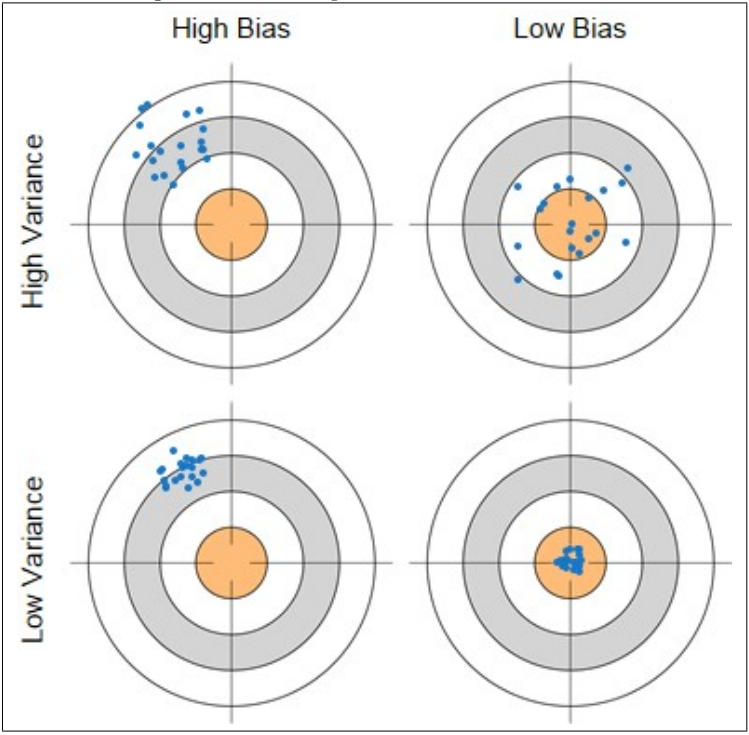
\includegraphics[height=.77\textheight]{slides3/bias_var.png}
    \caption{¿Cómo será el ECM en cada caso?}
  \end{figure}
\end{frame}


\begin{frame}{\color{rosee}(retomando la discusión: $\widehat{p}_{1}$ vs $\widehat{p}_{2}$) }
  \begin{exampleblock}{Estimar el par\'ametro de una Bernoulli}
    Volviendo al ejemplo, queremos comparar $\widehat{p}_{1}$ y $\widehat{p}_{2}$:
    % Volvamos al problema de estimar el $p$ de una Bernoulli. Nos
    % habiamos quedado con dos estimadores:
    \begin{itemize}
    \item[$\widehat{p}_{1}$] la media muestral:  
      \[\widehat{p_{1}}=\overline{X}_{n}\,.\]
    \item[$\widehat{p}_{2}$] agregar 2 fracasos y 2 \'exitos artificiales a la muestra y
      despues calcular la media muestral:
      \[\widehat{p}_{2} =  \frac{T + 2}{n+4}.\]
    \end{itemize}
    Calculemos el ECM de cada uno.
  \end{exampleblock}
\end{frame}

\begin{frame}{\color{rosee}(retomando la discusión: $\widehat{p}_{1}$ vs $\widehat{p}_{2}$)}
  \begin{exampleblock}{Estimar el par\'ametro de una Bernoulli}
    Sabemos que
    \begin{itemize}
    \item 
      \[E\left(\widehat{p}_{1}\right) = p\]
    \item 
      \[Var(\widehat{p}_{1})=\frac{p(1-p)}{n}\]
    \end{itemize}
    Entonces el ECM de $\widehat{p}_{1}$ es
    \[E\left[\left(\widehat{p}_{1}-p\right)^{2} \right]=\frac{p(1-p)}{n}.\]
  \end{exampleblock}
\end{frame}

\begin{frame}
Ustedes hacen las cuentas en clase para determinar el ECM de $\widehat{p}_{2}$. Ayudín: Recordá que la suma de $n$ v.a. independientes Bernoulli da como resultado una variable aleatoria Binomial. Por lo tanto: $T\sim Bin(n,p)$
\end{frame}

%\begin{frame}{\color{rosee}(retomando la discusión: $\widehat{p}_{1}$ vs $\widehat{p}_{2}$)}
%  \begin{exampleblock}{Estimar el par\'ametro de una Bernoulli}
%    Calculemos ahora el sesgo y la varianza de $\widehat{p}_{2}$. Notemos que 
%    que $T\sim Bin(n,p)$.
%    \[E\left( \frac{T+2}{n+4}
%    \right)-p=\frac{E(T+2)}{n+4}-p=\frac{np+2}{n+4}-p=\frac{2/n
%      -4p/n}{1+4/n}.\]
%    El sesgo no es cero, salvo cuando $p=0.5$. Sin embargo el sesgo
%    converge a cero cuando $n\to \infty$.
%    \[ Var\left( \frac{T+2}{n+4}
%    \right)=\frac{Var(T+2)}{(n+4)^{2}}=\frac{Var(T)}{(n+4)^{2}}=
%    \frac{np(1-p)}{(n+4)^{2}}.\]
%    Entonces
%    \[ E\left((\widehat{p}_{2}-p)^2\right)=\left(\frac{2/n
%        -4p/n}{1+4/n}\right)^2 + \frac{np(1-p)}{(n+4)^{2}}.\]
%  \end{exampleblock}
%\end{frame}

\begin{frame}{\color{rosee}(retomando la discusión: $\widehat{p}_{1}$ vs $\widehat{p}_{2}$)}
  \begin{exampleblock}{Estimar el par\'ametro de una Bernoulli}
    Tenemos
    \begin{align*}
      \text{ECM}(\widehat{p}_1,p) 
      &= E\left( (\widehat{p}_{1} - p)^{2} \right)=\frac{p(1-p)}{n}.\\ 
      \text{ECM}(\widehat{p}_2,p) 
      &= E\left( (\widehat{p}_{2} - p)^{2} \right)=
        \left(\frac{2/n -4p/n}{1+4/n}\right)^2
        + \frac{np(1-p)}{(n+4)^{2}}.
    \end{align*}
    ¿Cu\'al es mejor? 

    \bigskip Si uno de los dos ECM es m\'as bajo para todos los valores
    de $n$ y de $p$, ese ser\'ia el estimador deseable.

    \bigskip En la siguiente figura veremos que eso no pasa.
  \end{exampleblock}
\end{frame}

\begin{frame}{\color{rosee}(retomando la discusión: $\widehat{p}_{1}$ vs $\widehat{p}_{2}$)}\small
  \begin{figure}
    \centering
    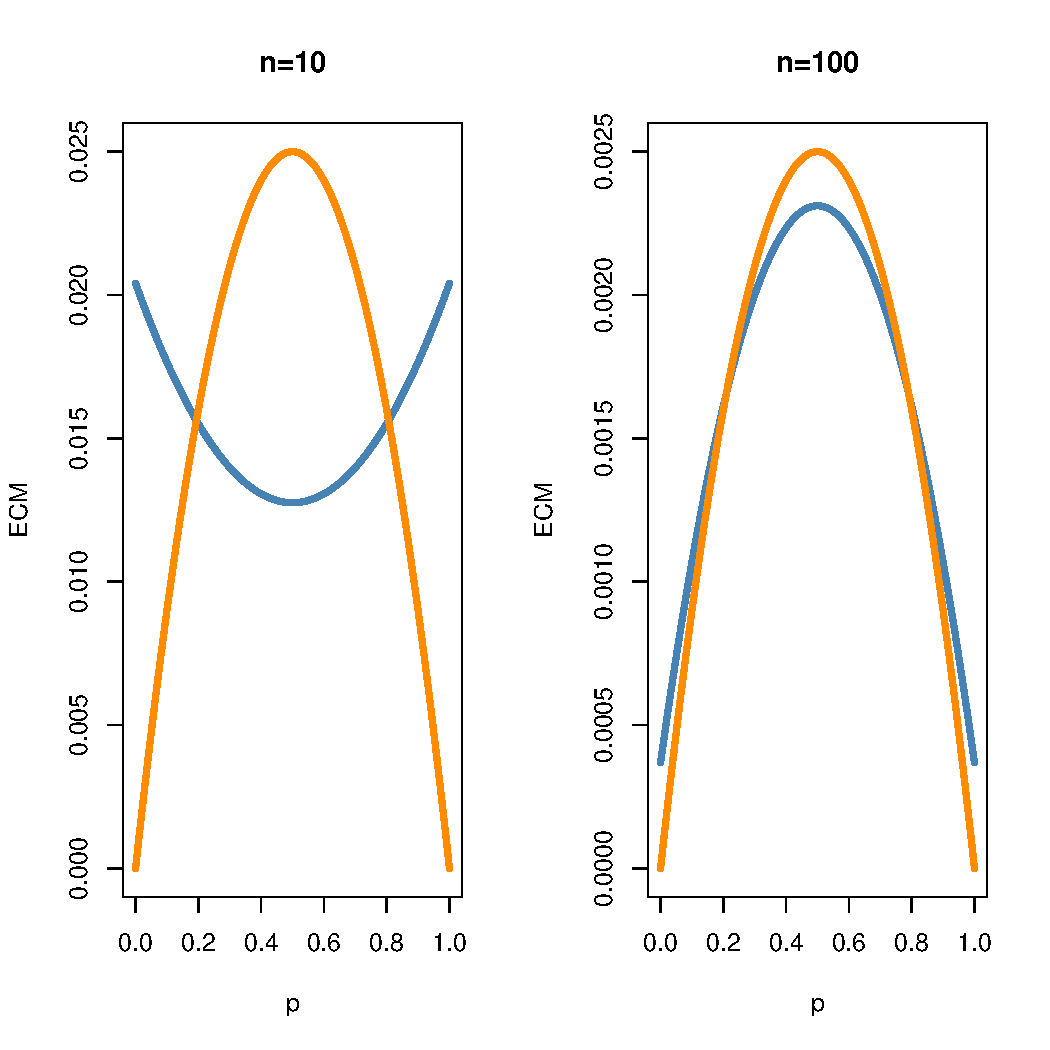
\includegraphics[height=.85\textheight]{slides3/ECM-bernoulli.pdf}
    \caption{Error cuadr\'atico medio para $\widehat{p}_{1}$ (naranja) y
      $\widehat{p}_{2}$ (azul).}
  \end{figure}
\end{frame}

\begin{frame}[fragile]{(¿lo querés replicar en R?)}
\begin{verbatim}
p = seq(0,1,by=0.01)
n = 10
ecm1 = p*(1-p)/n 
ecm2 = 4*(1-2*p)^2/(n+4)^2 + n/(n+4)^2*p*(1-p)

plot(p,ecm1, type = 'l', col = 'yellow',  
                     ylab ='ECM', xlab = 'p', lwd = 3)
points(p, ecm2, type = 'l', col = 'blue', lwd = 3)
\end{verbatim}
\medskip
\begin{itemize}
    \item ¿Qué ocurre con ambas curvas de ECM cuando $n\to \infty$?\medskip
    \item ¿Cómo interpetas este resultado? ¿Qué tiene que ver este resultado con lo que discutimos en la slide 11 de convergencia en probabilidad?\medskip
    \begin{itemize}
    \item \textit{Otra manera de probar consistencia}.
\end{itemize}
\end{itemize}
\end{frame}

\begin{frame}{\color{rosee}Error cuadr\'atico medio}
  \begin{block}{}
    \begin{itemize}
    \item Buscar un estimador que tenga un ECM que es menor que el de cualquier otro estimador, para cualquier valor posible del  par\'ametro a estimar, es demasiado ambicioso (en general este estimador no existe).\medskip
      
    \item Una manera de solucionar este dilema es restringir la clase (conjunto) de estimadores competidores. Una restricci\'on usual es la de quedarse \'unicamente con los estimadores insesgados.\medskip
    \begin{itemize}
        \item Sólo consideramos/evaluamos estimadores que pertenecen al conjunto de estimadores que \texti{en promedio} dicen \textit{la verdad}.\medskip
        \item Discutamos los detalles con mayor profundidad.
    \end{itemize}
    \end{itemize}
  \end{block}
\end{frame}

\begin{frame}{\color{rosee}Sesgo}
  \begin{definition}[Estimador insesgado]
    Un estimador $\widehat{\theta}_{n}$ de $\theta$ se dice \textbf{insesgado} si
    \[E(\widehat{\theta}_{n})=\theta\]
    para todos los valores posibles de $\theta$. En general, la diferencia 
    \[E(\widehat{\theta}_{n})-\theta\]
    se llama el \textbf{sesgo} del estimador.
  \end{definition}
  \begin{alertblock}{Intuición}
    $\widehat{\theta}_{n}$ es insesgado si, cualquiera sea el valor de $\theta$,
    la distribuci\'on muestral del estimador tiene centro de masa en
    $\theta$. \textbf{La propiedad de insesgadez, a diferencia de la de
      consistencia, no es un concepto asint\'otico.}
  \end{alertblock}
\end{frame}

\begin{frame}{\color{rosee}Algunos ejemplos:}
  \begin{exampleblock}{Ej I:}
    Si $\{X_{1},\dots,X_{n}\}$ es una muestra aleatoria con
$\mu=E(X_{1})=\dots=E(X_{n})$,  entonces $\overline{X}_{n}$ es un estimador insesgado de $\mu$.\\~\\~\\~\\~\\~\\~\\
  \end{exampleblock}

  \begin{exampleblock}{Ej II:}
    En el ejemplo que hicimos antes, $\widehat{p}_{2}$ result\'o ser un
    estimador sesgado de $\mu$.
  \end{exampleblock}
\end{frame}


\begin{frame}{\color{rosee}Reflexiones en torno a estimadores \textbf{insesgados}}
  \begin{itemize}
  \item Que un estimador sea insesgado no quiere decir que
    necesariamente esté \textit{cerca del par\'ametro verdadero}. Consideremos por ejemplo:
        \end{itemize}
    \begin{figure}
      \centering
    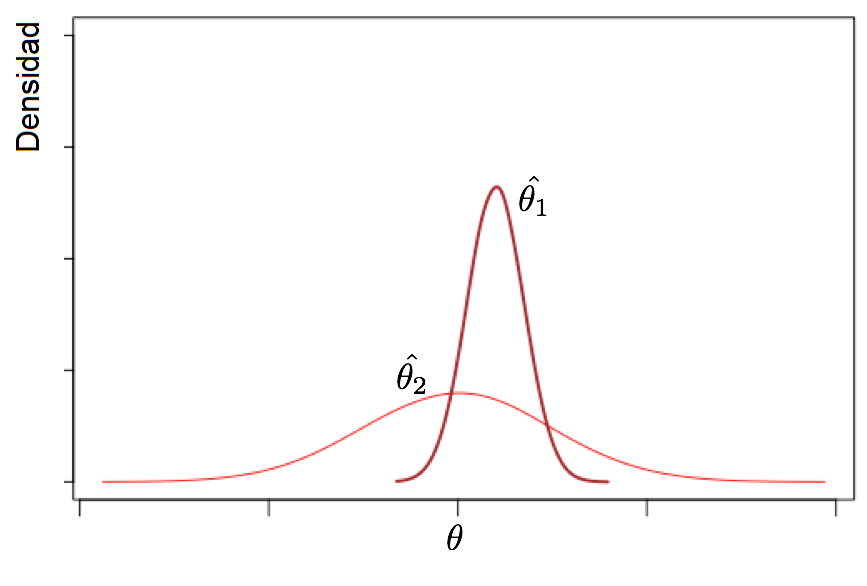
\includegraphics[height=.5\textheight]{slides3/biasvariance.png}
  \end{figure}
  \begin{itemize}
    \item El ECM s\'i mide en cierto sentido que un estimador est\'e cerca o lejos del par\'ametro de interés (discutimos un un ejemplo--ver slide 14-- de un estimador sesgado que puede ser mejor que otro insesgado, ya que para algunos valores del parámetro el primero tiene menor ECM).
 % \item Toda una \'area de la estad\'istica moderna estudia maneras
 %   inteligentes de balancear sesgo y varianza para tener un ECM bajo.
  \end{itemize}
\end{frame}

\begin{frame}{\color{rosee}Sesgo del estimador varianza muestral}\small
  \begin{exampleblock}{Ejemplo}
    Dada una muestra aleatoria $\{X_{1},\dots,X_{n}\}\stackrel{iid}{\sim} X$ con esperanza
    $E(X)= \mu$ y varianza $Var(X)=\sigma^{2}$; ya demostramos que si queremos estimar $\sigma^{2}$ entonces el estimador
    \[\widehat{\sigma}^{2}= \frac{1}{n}\sum\limits_{i=1}^{n}X_{i}^{2} -
    (\overline{X}_{n})^{2}\]
    es consistente. ¿Ser\'a insesgado?  Calculemos
    \[E\left[\frac{1}{n}\sum\limits_{i=1}^{n}X_{i}^{2} \right] \quad y
    \quad E\left[ (\overline{X}_{n})^{2}\right].\]
    La primera es f\'acil:
    \[E\left[\frac{1}{n}\sum_{i=1}^{n}X_{i}^{2} \right] =
    \frac{1}{n}\sum_{i=1}^{n}E(X_{i}^{2}) =
    E(X_{1}^{2})=\sigma^{2}+\mu^{2}.\]
  \end{exampleblock}
\end{frame}

\begin{frame}{\color{rosee}Sesgo del estimador varianza muestral}\small
  \begin{exampleblock}{Ejemplo}
    Ahora 
    \[E\left[ (\overline{X}_{n})^{2}\right]=Var(\overline{X}_{n}) +
    (E(\overline{X}_{n}))^{2}=\frac{\sigma^{2}}{n}+\mu^{2}.\] Luego
    \[ E(\widehat{\sigma}^{2})= \sigma^{2} + \mu^{2} -
    \frac{\sigma^{2}}{n} - \mu^{2}=\left(1 - \frac{1}{n}
    \right)\sigma^{2}\] y
    \[ E(\widehat{\sigma}^{2}) - \sigma^{2}= \frac{-\sigma^{2}}{n}.\]
    Por lo tanto, el estimador es sesgado: subestima el valor real.
  \end{exampleblock}
\end{frame}

\begin{frame}{\color{rosee}Sesgo del estimador CUASI--varianza muestral}\small
  \begin{exampleblock}{Ejemplo}
    Si consideramos ahora
    \[S^{2} = \frac{n}{n-1}\widehat{\sigma}^{2} =
    \frac{1}{n-1}\sum\limits_{i=1}^{n}(X_{i}-\overline{X}_{n})^{2}\]
    es f\'acil ver que $S^{2}$ es insesgado para $\sigma^{2}$.
  \end{exampleblock}
  
  % Pablo: hablamos ac\'a ya de la chi-cuadrado? para mostrar que un
  % sesgado puede tener menor ECM que un insesgado. En alg\'un lugar por
  % ac\'a, decir algo de medias podadas y robustez?

  % Lo dejar\'ia para m\'as adelante, me parece meter ruido. 

%  \begin{alertblock}{Comentarios}
%    \begin{itemize}
%    \item M\'as adelante, veremos que $S^2$ tiene distribuci\'on
%      $\chi^2_n$ (\textit{chi cuadrado con $n$ grados de libertad}).
%    \end{itemize}
%  \end{alertblock}
\end{frame}

\begin{frame}{\color{rosee}Comentarios y aclaraciones}
    \begin{itemize}
    \item Que $S^{2}$ sea insesgado para $\sigma^{2}$ no implica que $S$  sea insesgado para $\sigma$, de hecho no lo es.\medskip
    \item En general no es
      cierto que si $\widehat{\theta}_{n}$ es insesgado para $\theta$
      entonces $f(\widehat{\theta}_{n})$ es insesgado para $f(\theta)$.\medskip
    \item Un estimador puede ser sesgado y consistente a la vez  ($\widehat{\sigma}^{2}$). Un estimador puede ser insesgado y no ser consistente tambi\'en (¿por ejemplo?).\medskip
    \item ¿C\'ual deber\'iamos usar: $S^{2}$ (insesgado) o
      $\widehat{\sigma}^{2}$ (sesgado)? En la pr\'actica no importa mucho porque con $n$ relativamente grande las diferencias en los ECM de ambos son pequeñas.
    \end{itemize}
\end{frame}

\begin{frame}{\color{rosee}Ejemplos / Ejercicio en clase}\small
  \begin{exampleblock}{Ejemplo 1}
    Tenemos una muestra aleatoria $X_{1},\dots, X_{n}$ con densidad
    \[f(x)=\frac{1}{2} (1+\theta x) \, I_{(-1,1)}(x)\,.\]
    Muestre que $3 \overline{X}_{n}$ es un estimador insesgado y
    consistente de $\theta$.
  \end{exampleblock}
%  \begin{exampleblock}{Ejemplo 2}
%    Un tipo de fertilizante tiene un rinde esperado por hect\'area igual
%    a $\mu_{1}$ con una varianza igual a $\sigma^{2}$, mientras que otro
%    fertilizante tiene un rinde esperado por hect\'area igual a
%    $\mu_{2}$ con una varianza igual a $\sigma^{2}$. 
%    
%    \bigskip Sean $S_{1}^{2}$ y
%    $S_{2}^{2}$ los desv\'ios est\'andar muestrales basados en muestras
%    de tama\~no $n_1$ y $n_2$ respectivamente para los dos
%    fertilizantes. Proponga un estimador insesgado de $\sigma^{2}$.
%  \end{exampleblock}
\end{frame}

\begin{frame}%{Sesgo}\small
  \begin{exampleblock}{Ejemplo 2}
    Vimos que si $X\sim Unif(0,\theta)$, dada una muestra aleatoria
    $X_{1},\dots,X_{n}$, un estimador consistente de $\theta$ es
    \[\widehat{\theta}_{n}=\max(X_{1},\dots, X_{n}).\]
    Vimos que
    \[ E \left(\widehat{\theta}_{n}\right)=\frac{n}{n+1}\theta,\]
    as\'i que $\widehat{\theta}_{n}$ no es insesgado. 
    
    \medskip ¿C\'omo lo corregimos para que sea insesgado? Es f\'acil
    ver que
    \[\widetilde{\theta}_{n} = \frac{n+1}{n} \widehat{\theta}_{n}\]
    es insesgado. Tambien es f\'acil ver que $2{\overline{X}_{n}}$
    es insesgado. ¿Con cu\'al nos quedamos?
  \end{exampleblock}
\end{frame}

\begin{frame}{\color{rosee}M\'inima varianza}
  \begin{definition}[Eficiencia relativa]
    Dados dos estimadores \unterline{insesgados} $\widehat{\theta}_{n}$ y
    $\widetilde{\theta}_{n}$ de $\theta$, decimos que $\widehat{\theta}_{n}$ es
    m\'as \textbf{eficiente} que $\widetilde{\theta}_{n}$ si
    \[Var(\widehat{\theta}_{n}) \leq Var(\widetilde{\theta}_{n}).\]
  \end{definition}
  \begin{alertblock}{Idea}
    Si $\widehat{\theta}_{n}$ es m\'as eficiente que
    $\widetilde{\theta}_{n}$, entonces $\widehat{\theta}_{n}$ usa mejor la  informaci\'on en la muestra que $\widetilde{\theta}_{n}$. Notar también que si $\widehat{\theta}_{n}$ es más eficiente que $\widetilde{\theta}_{n}$, entonces el ECM del primer estimador es menor que el del segundo estimador.
  \end{alertblock}
\end{frame}

%\begin{frame}{\color{rosee}M\'inima varianza}
%  % Pablo: un grafiquito, dos densidades centradas en theta una m\'as
%  % dispera que la otra
%  \begin{figure}
%    \centering
%    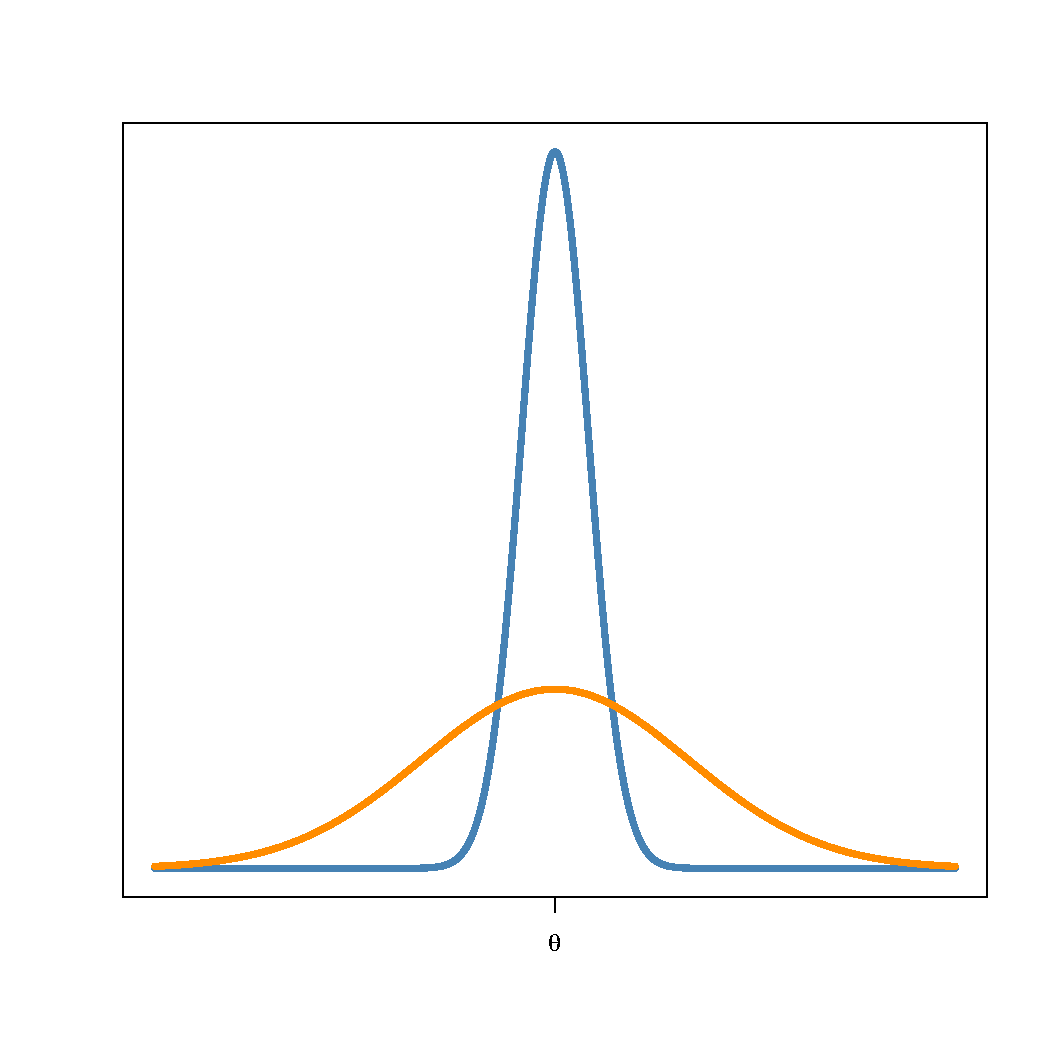
\includegraphics[height=\textheight]{figs/eficiencia.pdf}
%  \end{figure}
%\end{frame}

\begin{frame}{\color{rosee}M\'inima varianza (ejemplos)}\small
  \begin{exampleblock}{El modelo uniforme}
    Ya vimos que $2{\overline{X}_{n}}$ y
    $\frac{n+1}{n} \widehat{\theta}_{n}$ son insesgados. Notemos que
    \[Var\left(\frac{n+1}{n}
      \widehat{\theta}_{n}\right)=\left(\frac{n+1}{n}
    \right)^{2}Var(\widehat{\theta}_{n}) = \frac{\theta^{2}}{n(n+2)}.\]
    Por otro lado,
    \[Var\left(2{\overline{X}_{n}}\right)=4 Var(\overline{X}_{n}) =
    \frac{4}{n} Var(X_{1})=\frac{4}{n} \frac{\theta^{2}}{12} =
    \frac{\theta^2}{3n}\]
    Para todo $n>1$ y para todo $\theta$
    \[\frac{\theta^{2}}{n(n+2)} \leq \frac{\theta^{2}}{3n}\,.\]
  \end{exampleblock}
\end{frame}

\begin{frame}{\color{rosee}M\'inima varianza}\small
  \begin{exampleblock}{Ejemplo}
    Entonces concluimos que 
    \[\widetilde{\theta}_{n} = \frac{n+1}{n} \widehat{\theta}_{n}\]
    es m\'as eficiente que $2{\overline{X}_{n}}$. Luego, preferimos
    $\widetilde{\theta}_{n} $. 

    \bigskip Notemos que para valores de $n$ grande, la varianza de
    $\widetilde{\theta}_{n}$ es mucho m\'as chica que la de
    $2{\overline{X}_{n}}$. De hecho
    \[\frac{Var(\widetilde{\theta}_{n})}{Var(2{\overline{X}_{n}})} \ton 0.\]
  \end{exampleblock}
\end{frame}

\begin{frame}{\color{rosee}M\'inima varianza} \small
  \begin{definition}[IMV]
    Entre todos los estimadores de $\theta$ que son insesgados, el que
    tiene m\'inima varianza se denomina \textbf{estimador insesgado de
      m\'inima varianza (IMV)}.
  \end{definition}
  \begin{alertblock}{Idea}
    El IMV es, de todos los insesgados, el que tiene una distribuci\'on
    muestral con menor dispersi\'on alrededor de $\theta$. Entonces,
    como sabemos que el ECM es la suma de la varianza del estimador y de
    su sesgo al cuadrado, el estimador IMV es el que minimiza el ECM
    entre los insesgados.
  \end{alertblock}
\end{frame}

\begin{frame}{\color{rosee}M\'inima varianza}\small
  \begin{proposition}
    Sea $\{X_{1},\dots, X_{n}\}\stackrel{iid}{\sim} X$ una muestra aleatoria de una \underline{distribuci\'on
    normal} con par\'ametros $\mu$ y $\sigma^{2}$ ($X\sim N(\mu,\sigma^2)$). Entonces
    $\overline{X}_{n}$ es el estimador IMV de $\mu$.
  \end{proposition}
  \begin{alertblock}{Ojo}
    Es clave en esta proposici\'on la \textbf{hip\'otesis de normalidad}. Si los
    datos no son normales, $ \overline{X}_{n}$ no tiene porqu\'e ser el IMV para estimar $E(X)=\mu$.
  \end{alertblock}
  \begin{exampleblock}{Ejemplo (uniforme)}
    Para la uniforme, se puede mostrar que
    \[\widetilde{\theta}_{n} = \frac{n+1}{n} \max(X_{1},\dots,X_{n})\]
    es el estimador IMV (antes solo hab\'iamos mostrado que es m\'as
    eficiente que $2\overline{X}_{n}$).
  \end{exampleblock}
\end{frame}

\begin{frame}{\color{rosee}M\'inima varianza}\small
No vamos a ver en el curso como obtener estimadores IMV en general.

\bigskip

Más adelante estudiaremos una familia de estimadores que tienen mínima
varianza \textbf{asintótica}, que es el tipo de `optimalidad' relevante
para construir intervalos de confianza y tests de hipótesis.
\end{frame}

\begin{frame}{\color{rosee}Error est\'andar}\small
  Adem\'as de reportar la estimaci\'on (puntual) debemos indicar su
  precisi\'on.
  \begin{definition}[Error est\'andar]
    El \textbf{error est\'andar} de un estimador $\widehat{\theta}_{n}$
    es otro nombre para el desv\'io est\'andar de su distribuci\'on:
    $\sqrt{Var(\widehat{\theta}_{n})}$.
  \end{definition}
  \begin{alertblock}{Idea}
    \begin{itemize}
    \item El error est\'andar mide la variabilidad del estimador. Si
      repetimos el experimento, cambia la muestra y posiblemente cambie
      el valor estimado. Necesitamos una idea de qu\'e tan estable es el
      estimador.
    \item En algunos casos podremos calcularlo exactamente y en otros,
      la mayor\'ia, tendremos que estimarlo.
    \end{itemize}
  \end{alertblock}
\end{frame}

\begin{frame}{\color{rosee}Error est\'andar} \small
  \begin{exampleblock}{Ejemplo}
    El error est\'andar de $\overline{X}_{n}$ es
    \[\sqrt{Var\left(\overline{X}_{n}\right)}= \frac{\sqrt{Var(X)}}{\sqrt{n}}.\]
    Un estimador consistente de $\sqrt{Var(X)}$ es
    \[\widehat{\sigma}= \sqrt{\frac{1}{n} \sum_{i=1}^{n}X_{i}^{2}
      - \left(\overline{X}_{n}\right)^{2}}\]
    otro es
    \[S= \widehat{\sigma} \sqrt{\frac{n}{n-1}}.\]
    Luego, podemos estimar el error est\'andar de $\overline{X}_{n}$ con
    $\frac{\widehat{\sigma}}{\sqrt{n}}$.
  \end{exampleblock}
\end{frame}

\begin{frame}{\color{rosee}{Error est\'andar}} \small
  \begin{exampleblock}{Ejemplo}
    Vimos adem\'as, usando el TCL y el Lema de Slutsky, que
    \[ \sqrt{n}\, \frac{(\overline{X}_{n} - \mu)}{\widehat{\sigma}}
    \sim_a N\left(0, 1\right) 
    \quad\mbox{y}\quad \overline{X}_{n} - \mu \sim_a N\left(0, \frac{\widehat{\sigma}^{2}}{n}\right).\] Por lo tanto, si $Z\sim N(0,1)$:
    \[ P\left( \left\vert \overline{X}_{n} - \mu \right\vert \leq
      2\underbrace{\frac{\widehat{\sigma}}{\sqrt{n}}}_{\text{Er. Std.}}\right) \approx P\left(
      \left\vert Z \right\vert \leq 2 \right) \approx 0.95.\]
    Con probabilidad aproximadamente 0.95, $\overline{X}_{n}$ se realiza a lo sumo a una distancia menor o igual que dos
    errores est\'andar (estimados) del par\'ametro verdadero $\mu$.
    
    \bigskip \textbf{¡Esto habla sobre ninguna realizaci\'on particular del
      experimento!}
  \end{exampleblock}
\end{frame}

% \begin{frame}{\color{rosee}Error est\'andar}\small
%   \begin{exampleblock}{Ejemplo}
%     \bigskip ¿Qu\'e quiere decir esto? Si $n$ es `grande' y repetimos
%     muchas veces el experimento de tomar una muestra y calcular
%     $\overline{X}_{n}$, aproximadamente en el 95\% de las repeticiones,
%     el valor de la media muestral calculada estar\'a a una distancia
%     menor o igual que dos desv\'ios est\'andars estimados del
%     par\'ametro verdadero.

%     \bigskip \textbf{Esto no dice nada sobre ninguna realizaci\'on del
%       experimento en particular!}
%   \end{exampleblock}
% \end{frame}

\begin{frame}{\color{rosee}Error est\'andar}\small
  \begin{exampleblock}{Ejemplo}
    En el proceso de ensamblaje de celulares en una f\'abrica se cometen
    errores. El n\'umero de rayaduras en la pantalla de un celular
    elegido al azar de la l\'inea de montaje es una variable aleatoria
    $X$ con distribuci\'on Poisson de par\'ametro $\lambda$. Se toma una
    muestra aleatoria de $150$ celulares y se registran los siguientes
    resultados:
% , donde la primer fila indica el n\'umero de rayaduras y
%     la segunda la frecuencia observada. Por ejemplo, hubo 42 celulares
%     en la muestra con 2 rayaduras en la pantalla.
    \begin{table}
      \centering
      \begin{tabular}{|r|rrrrrrrr|}
        \hline
        \mbox{n\'umero de rayaduras}&0&1&2&3&4&5&6&7\\
        \mbox{ocurrencias en la muestra}&18&37&42&30&13&7&2&1\\
        \hline
      \end{tabular}
    \end{table}
    \begin{itemize}
    \item Proponga un estimador consistente e insesgado para
      $\lambda$. Calcule el valor estimado obtenido para esta muestra.
    \item Proponga un estimador consistente para la varianza
      de $X$. Proponga un estimador para el error est\'andar del
      estimador propuesto en el item anterior. ¿C\'ual es el error
      est\'andar estimado para esta muestra?
    \end{itemize}
  \end{exampleblock}
\end{frame}
%\end{document} %%% Después decido si alargo las diapos o pongo dos filminas diferentes.
\section{Modelos Paramétricos y Método de Momentos}

\begin{frame}{\color{rosee}Modelos param\'etricos}
  \begin{alertblock}{Notaci\'on}
    A continuación usaremos la palabra densidad para referirnos tanto a
    la densidad de variables/vectores aleatorios continuos como a la
    funci\'on de probabilidad puntual de variables/vectores aleatorios
    discretos.
  \end{alertblock}
\end{frame}

\begin{frame}{\color{rosee}Modelos param\'etricos}
  \begin{definition}[Modelo param\'etrico]
    Supongamos que tenemos una muestra aleatoria $X_{1},\dots,X_{n}$ con
    cierta funci\'on de densidad $f$. Un \textbf{modelo param\'etrico}
    para la distribuci\'on de la muestra aleatoria es postular que $f$
    pertenece un conjunto de funciones de densidad que depende de un
    par\'ametro desconocido $\theta$:
    \[f \in \left\{ f(x)=f(x;\theta) \text{ para cierto
      }\theta\right\},\]
    donde la forma de las funciones $f(x;\theta)$ es completamente
    conocida, excepto por $\theta$.
  \end{definition}
  \begin{alertblock}{Idea}
    Suponer un modelo param\'etrico para una muestra aleatoria es
    suponer que conocemos enteremante la distribuci\'on de los datos,
    \textbf{excepto por una cantidad finita de par\'ametros}.
  \end{alertblock}
\end{frame}



\begin{frame}{\color{rosee}Modelos param\'etricos}\small
  Ya vimos mucho modelos param\'etricos (sin haberlos llamado as\'i)
  \begin{exampleblock}{Ejemplo 1}
    Tenemos una muestra aleatoria $X_{1},\dots, X_{n}$ con densidad
    \[f(x)=1/2 (1+\theta x) I_{(-1,1)}(x)\]
  \end{exampleblock}
  \begin{exampleblock}{Ejemplo 2}
    Supongamos que el tiempo de reacci\'on de una persona intoxicada a
    cierto est\'imulo es una variable aleatoria $X$, que tiene
    distribuci\'on uniforme en el intervalo $(0, \theta)$ para un valor
    de $\theta$ desconocido. Tenemos una muestra aleatoria
    $X_{1},\dots, X_{n}$ y queremos estimar $\theta$.
  \end{exampleblock}
  \begin{exampleblock}{Ejemplo 3}
    Suponer que los datos provienen de una normal con par\'ametros
    desconocidos, o de una Poisson con par\'ametro desconocido tambi\'en
    son modelos param\'etricos.
  \end{exampleblock}
\end{frame}

\begin{frame}{\color{rosee}Modelos param\'etricos}
  \begin{block}{}
    Los modelos \textbf{no param\'etricos} son aquellos que no ponen
    restricciones param\'etricas a la distribuci\'on que suponemos
    tienen los datos.
    
    \bigskip El siguiente es un ejemplo de un modelo no-param\'etrico,
    pero solo nos interesa estimar ciertos par\'ametros de la
    distribuci\'on.
  \end{block}
  \begin{exampleblock}{Ejemplo}
    Nos interesa estudiar el estado de salud de la poblaci\'on
    Argentina, en particular su peso. Supongamos que el peso de una
    persona elegida al azar es una variable aleatoria con esperanza
    $\mu$ y varianza $\sigma^{2}$ desconocidos. A partir de una muestra
    aleatoria de pesos $X_{1},\dots,X_{n}$ queremos estimar $E(X)$ y
    $Var(X)$.
  \end{exampleblock}
\end{frame}

\begin{frame}{\color{rosee}Modelos param\'etricos}
  % PABLO: Un ejemplo no rebuscadisimo de esto?
  Los siguientes ejemplos son modelos no param\'etrico, nos interesa
  estimar una funci\'on entera que depende de la distribuci\'on m\'as
  que una \'unica caracter\'istica num\'erica.
  \begin{exampleblock}{Ejemplo}
    \begin{itemize}
    \item Estimar \textbf{toda} la funci\'on de distribuci\'on acumulada
      del ingreso anual de una poblaci\'on. A partir de la estimaci\'on
      podemos obtener estimaciones de diferentes cuantiles.
    \end{itemize}
  \end{exampleblock}
\end{frame}

\begin{frame}{\color{rosee}Modelos param\'etricos}\small
  \begin{block}{Modelos param\'etricos}
    Los modelos param\'etricos hacen suposiciones muy fuertes. Suponen
    que conocemos pr\'acticamente todo sobre c\'omo se generan los
    datos.
  \end{block}
  \begin{block}{¿C\'uando es razonable un modelo param\'etrico?}
    Depende\dots
    \begin{itemize}
      % Pablo: (tecnecio?, Pablo referencia?)
    \item En algunos problemas f\'isicos o de ingenier\'ia, hay
      experimentos duros que validan el modelado de ciertas cantidades
      aleatorias de manera param\'etrica. Un ejemplo: como emite
      radiaci\'on un \'atomo inestable sigue una distribuci\'on Poisson.
    \item En problemas socioecon\'omicos, es m\'as d\'ificil creerse que
      valga exactamente un modelo param\'etrico.
    \end{itemize}
  \end{block}
\end{frame}

\begin{frame}{\color{rosee}Modelos param\'etricos}
George P. Box: ``All models are wrong, but some are
      useful.''
\end{frame}

\begin{frame}{\color{rosee}Modelos param\'etricos}
  Aunque un modelo param\'etrico no valga exactamente, si vale
  ``aproximadamente'' puede ser \'util para \textbf{aprender} de los datos.
  
  \bigskip
  \begin{center}
    ¿C\'omo sabemos si un modelo param\'etrico es razonable?
  \end{center}

\bigskip

  Esto escapa al alcance de esta materia, pero veamos algunas ideas en un ejemplo simple:
\end{frame}



\begin{frame}{\color{rosee}Ejemplo: Containers perdidos}
  % FUENTE:
  % https://www.math.psu.edu/treluga/textbook/fitting_distributions.html

 \small{Tenemos información sobre el número de containers que pierde cada año una empresa de logística internacional en cada uno de sus 16 centros de distribución.}

  \tiny
  \renewcommand{\arraystretch}{1.2}
  \begin{table}
    \centering
    \begin{tabular}{cccccccccccccccc}
      A\~no&C0&C1&C2&C3&C4&C5&C6&C7&C8&C9&C10&C11&C14&C15\\
      \hline
      1975&0&0&0&0&0&0&0&1&1&0&0&0&1&0\\
      1976&2&0&0&0&1&0&0&0&0&0&0&0&1&1\\
      1977&2&0&0&0&0&0&1&1&0&0&1&0&2&0\\
      1978&1&2&2&1&1&0&0&0&0&0&1&0&1&0\\
      1979&0&0&0&1&1&2&2&0&1&0&0&2&1&0\\
      1980&0&3&2&1&1&1&0&0&0&2&1&4&3&0\\
      1981&1&0&0&2&1&0&0&1&0&1&0&0&0&0\\
      1982&1&2&0&0&0&0&1&0&1&1&2&1&4&1\\
      1983&0&0&1&2&0&1&2&1&0&1&0&3&0&0\\
      1984&3&0&1&0&0&0&0&1&0&0&2&0&1&1\\
      1985&0&0&0&0&0&0&1&0&0&2&0&1&0&1\\
      1986&2&1&0&0&1&1&1&0&0&1&0&1&3&0\\
      1987&1&1&2&1&0&0&3&2&1&1&0&1&2&0\\
      1988&0&1&1&0&0&1&1&0&0&0&0&1&1&0\\
      1989&0&0&1&1&0&1&1&0&0&1&2&2&0&2\\
      1990&1&2&0&2&0&1&1&2&0&2&1&1&2&2\\
      1991&0&0&0&1&1&1&0&1&1&0&3&3&1&0\\
      1992&1&3&2&0&1&1&3&0&1&1&0&1&1&0\\
      1993&0&1&0&0&0&1&0&2&0&0&1&3&0&0\\
      1994&1&0&0&0&0&0&0&0&1&0&1&1&0&0
    \end{tabular}
  \end{table}
\end{frame}

\begin{frame}{\color{rosee}Ejemplo: Containers perdidos}\small
  \begin{columns}
    \begin{column}{.6\textwidth}
      \begin{figure}
        \centering
        \includegraphics[height=.8\textheight]{slides3/hist-soldados-poisson.pdf}
      \end{figure}
    \end{column}
    \begin{column}{.3\textwidth}
      Veamos la distribuci\'on del n\'umero de containers perdidos por centro de distribución,
      por a\~no.
      \begin{table}
        \centering
        \begin{tabular}{c| c}
          0& 144\\
          1& 91 \\
          2& 32 \\
          3& 11 \\
          4& 2 \\
          5& 0 \\
          6& 0 \\
          7& 0 
        \end{tabular}
        % \caption{Muertes anuales por patadas de caballo en el
        % ej\'ercito Prusiano (1875-1894)}
      \end{table}
    \end{column}
  \end{columns}
\end{frame}

\begin{frame}{\color{rosee}Ejemplo: Containers perdidos}\small
  \begin{columns}
    \begin{column}{.45\textwidth}
      \begin{figure}
        \centering
        \includegraphics[height=.8\textheight]{slides3/hist-soldados-poisson.pdf}
      \end{figure}
    \end{column}
    \begin{column}{.45\textwidth}
      Ajustamos una distribuci\'on Poisson de par\'ametro
      $\lambda = 0.7$.
    \end{column}
  \end{columns}
\end{frame}

\begin{frame}{\color{rosee}M\'etodos de estimaci\'on}\small
  \begin{block}{M\'etodos de estimaci\'on}
    Hasta ahora hemos obtenido estimadores a trav\'es de argumentos
    intuitivos.  A continuaci\'on, estudiaremos \textbf{m\'etodos} para
    construir estimadores en problemas generales: dada una muestra
    $X_{1},\dots, X_{n}$ y un par\'ametro $\theta$ asociado a la
    distribuci\'on de la muestra, ¿c\'omo podemos estimar $\theta$?
    \begin{itemize}
    \item m\'etodo de los momentos
    \item m\'etodo de m\'axima verosimilitud
    \end{itemize}
  \end{block}
\end{frame}

\begin{frame}{\color{rosee}M\'etodo de los momentos} \small
  \begin{definition}[Momento poblacional]
    Para $k\in\mathbb{N}$, se define el $k$-\'esimo \textbf{momento
      poblacional} de la variable aleatoria $X$ como
    $E\left(X^{k}\right)$.
  \end{definition}
  \begin{definition}[Momento muestral]
    Dada una muestra aleatoria con la misma distribuci\'on que $X$. Se
    define el $k$-\'esimo \textbf{momento muestral} de
    $X_{1},\dots,X_{n}$ como $\frac{1}{n}\sum_{i=1}^{n}X_{i}^{k}$.
  \end{definition}
  \begin{block}{}
    \begin{itemize}
    \item El primer momento poblacional es $E(X)$.
    \item El primer momento muestral es $\overline{X}_{n}$, la media
      muestral.
    \item El segundo momento poblacional es $E(X^2)$. 
    \item El segundo momento muestral es $\frac{1}{n}\sum_{i=1}^{n}X_{i}^{2}$.
    \end{itemize}
    Notar que los momentos poblacionales son n\'umeros fijos, y los
    muestrales son variables aleatorias.
  \end{block}
\end{frame}

\begin{frame}{\color{rosee}M\'etodo de los momentos}\small
  \begin{definition}[M\'etodo de los momentos]
    Sea $X_1,\dots,X_n$ una muestra aleatoria con densidad $f(x;\theta)$
    donde $\theta=(\theta_1,\dots,\theta_m)$ son par\'ametros
    desconocidos. Supongamos que los primeros $m$ momentos poblacionales
    son funciones de $\theta_{1},\dots,\theta_{m}$, es decir que para
    $k=1,\dots,m$
    \[ E\left(X^{k}\right)=g_{k}(\theta_{1},\dots,\theta_{m}).\]
    Los estimadores del m\'etodo de los momentos
    $\widehat{\theta}^{(1)}_{MM},\dots,\widehat{\theta}^{(m)}_{MM}$ son
    los que se obtienen de igualar los primeros $m$ momentos muestrales
    a los poblaciones y despejar $\theta_{1},\dots,\theta_{m}$. Es
    decir, de resolver conjuntamente para $k=1,\dots,m$.
    \[g_{k}\left(\widehat{\theta}^{(1)}_{MM},\dots,\widehat{\theta}^{(m)}_{MM}\right)=
    \frac{1}{n}\sum_{i=1}^{n}X_{i}^{k}\]
  \end{definition}
\end{frame}

\begin{frame}{\color{rosee}M\'etodo de los momentos}
  \begin{alertblock}{Notaci\'on}
  En $\widehat{\theta}_{MM}$ omitimos el sub\'indice $n$ que indica el
  tama\~no de muestra para no sobrecargar la notaci\'on.
\end{alertblock}
\end{frame}

\begin{frame}{\color{rosee}M\'etodo de los momentos}
  \begin{exampleblock}{Estimador de momentos para la Bernoulli}
    Sea $X_{1},\dots,X_{n}$ una muestra aleatoria con distribuci\'on
    $Ber(p)$. El estimador de momentos de $\theta=p$ se obtiene de la
    siguiente manera. El primer momento de una $Ber(p)$ (su esperanza)
    es igual a $p$. 
    Luego el estimador es
    \[\widehat{\theta}_{MM}=\frac{1}{n}\sum\limits_{i=1}^{n}X_{i}.\]
    Es decir, el estimador es la media muestral.
  \end{exampleblock}
\end{frame}


\begin{frame}{\color{rosee}M\'etodo de los momentos}
\begin{exampleblock}{Ejemplo}
Sea $X_{1},\dots,X_{n}$ una muestra aleatoria con distribución $Ber(p)$. Calcular el estimador de momentos de las odds, $p/(1-p)$.
\end{exampleblock}
\end{frame}

\begin{frame}{\color{rosee}M\'etodo de los momentos}
  \begin{exampleblock}{Estimador de momentos para la normal}
    Sea $X_{1},\dots,X_{n}$ una muestra aleatoria con distribuci\'on
    $N(\mu, \sigma^{2})$.  
    
    \bigskip Calculemos el estimador de momentos de
    $\theta=(\mu, \sigma^{2})$. Tenemos que resolver
    \begin{align*}
      E(X_1)&=\frac{1}{n}\sum\limits_{i=1}^{n}X_{i}\\
      E\left(X_{1}^{2}\right)&=\frac{1}{n}\sum\limits_{i=1}^{n}X_{i}^{2}.
    \end{align*}
    Sabemos que $E(X_1)=\mu$ y $E(X_{1}^{2})=\sigma^{2}+\mu^{2}$.
  \end{exampleblock}
\end{frame}

\begin{frame}{\color{rosee}M\'etodo de los momentos}
  \begin{exampleblock}{Estimador de momentos para la normal}
    Luego
    \begin{align*}
      \widehat{\mu}_{MM}&=\frac{1}{n}\sum_{i=1}^{n}X_{i}\\
      \widehat{\sigma}_{MM}^{2}+\widehat{\mu}_{MM}^{2}&=\frac{1}{n}\sum_{i=1}^{n}X_{i}^{2}.
    \end{align*}
    y por lo tanto el estimador de momentos de $\mu$,
    $\widehat{\mu}_{MM}$, es igual a $\overline{X}_{n}$ y el estimador
    de momentos de $\sigma_{2}$ es
    \[\widehat{\sigma}_{MM}^{2}=\frac{1}{n}\sum_{i=1}^{n}X_{i}^{2}
    - (\overline{X}_{n})^{2},\]
    que es el estimador $\widehat{\sigma}^{2}$ que ya hab\'iamos
    estudiado antes.
  \end{exampleblock}
\end{frame}

\begin{frame}{\color{rosee}M\'etodo de los momentos}
  \begin{exampleblock}{Ejemplo}
    Sea $X$ el tiempo que dedica un alumno a estudiar para un
    examen. Supongamos que la densidad de $X$ es
    \[f(x;\theta)=(\theta+1)x^{\theta} I_{(0,1)}(x)\]
    y que sabemos que $\theta>-1$. 
    
    \bigskip Calcule el estimador de momentos de $\theta$ y dar el valor
    estimado para la siguiente muestra:
    \begin{align*}
      x_{1}&=0.92, x_{2}=0.79, x_{3}=0.90,x_{4}=0.65, x_{5}=0.86,\\
      x_{6}&=0.47, x_{7}=0.73, x_{8}=0.97, x_{9}=0.94, x_{10}=0.77
    \end{align*}
  \end{exampleblock}
\end{frame}



\begin{frame}{\color{rosee}Variable aleatoria exponencial}
  \begin{definition}[Variable exponencial]
    Decimos que una variable aleatoria continua $X$ tiene
    \textbf{distribuci\'on exponencial} de par\'ametro $\lambda>0$ si su
    funci\'on de densidad es
    \[f(x;\lambda)=\lambda e^{-\lambda x} I_{(0,+\infty)}(x)\,.\]
  \end{definition}
  \begin{block}{Notaci\'on}
    Usaremos la notaci\'on $X\sim Exp(\lambda)$.
  \end{block}
\end{frame}

\begin{frame}{\color{rosee}Variable aleatoria exponencial}
  \begin{figure}
    \centering
    \includegraphics[height=.85\textheight]{slides3/exponencial.pdf}
    \caption{Densidad de la distribuci\'on exponencial para diferentes
      $\lambda$.}
  \end{figure}
\end{frame}

\begin{frame}{\color{rosee}Variable aleatoria exponencial}\small
  Las variables exponenciales se suelen usar para modelar tiempos de
  espera entre `eventos', por ejemplo:
  \begin{itemize}
  \item el tiempo que pasa entre que llegan dos llamadas a un call--center.
  \item el tiempo que pasa entre que llegan dos clientes a un local.
  \end{itemize}
  Se usan variables exponenciales para modelar este tipo de problemas,
  parte por el siguiente resultado
  \begin{proposition}[Conexi\'on con la distribuci\'on Poisson]
    Supongamos que el n\'umero de eventos que ocurren en cualquier
    intervalo de longitud $t$ tiene distribuci\'on Poisson con par\'ametro
    $\lambda t$ y que adem\'as el n\'umero de eventos que ocurren en
    intervalos de tiempo disjuntos son independientes. Entonces el tiempo
    que pasa entre dos eventos es una variable aleatoria exponencial de
    par\'ametro $\lambda$.
  \end{proposition}
\end{frame}

\begin{frame}{\color{rosee}Variable aleatoria exponencial}\small
  \begin{block}{}
    Otro uso de las variables exponenciales es para modelar el tiempo de
    vida de partes de un sistema, por ejemplo, el tiempo hasta que se
    quema una lamparita. Esto se debe en parte a la siguiente propiedad
    de la exponencial.
  \end{block}
  \begin{proposition}[P\'erdida de memoria]
    Sea $X\sim Exp(\lambda)$. Entonces, si $t, t_0 >0$
    \[P\left( X \geq t+ t_{0}\mid X\geq t_{0}\right) =P\left( X \geq
      t\right) = e^{-\lambda t}.\]
  \end{proposition}
  \begin{alertblock}{Idea}
    Si ya sabemos que la lamparita dur\'o $t_0$ d\'ias, la probabilidad
    de que dure al menos $t$ d\'ias m\'as es igual a la probabilidad
    (incondicional) de que la lamparita dure al menos $t$ d\'ias. El
    tiempo que le queda de funcionamiento a la lamparita es
    independiente de cuando tiempo de uso lleva.
  \end{alertblock}
\end{frame}

\begin{frame}{\color{rosee}Variable aleatoria exponencial}\small
  \begin{proof}
    Si $t>0$
    \[P\left( X \leq t\right) = \int_{0}^{t} \lambda e^{-\lambda x}
    \, dx=-e^{-\lambda x} \vert_{0}^{t}= 1 - e^{-\lambda t}\,.\] Luego,
    \[P\left( X \geq t\right) = 1 - P\left( X < t\right) = 1 - \left(1 -
    e^{-\lambda t}\right) = e^{-\lambda t}.\] Entonces,
    \begin{align*}
      P\left( X \geq t+ t_{0}\mid X\geq
      t_{0}\right)&=\frac{P\left(\{ X \geq t+ t_{0} \}\cap
        \{ X\geq t_{0} \}\right)}{P\left(X\geq t_0 \right)}\\
      &= \frac{P\left(\{ X \geq t+ t_{0}
      \}\right)}{P\left(X\geq t_0 \right)}
      =\frac{e^{-\lambda(t+t_0)}}{e^{-\lambda t_0}}=e^{-\lambda t}.
    \end{align*}
  \end{proof}
\end{frame}

\begin{frame}{\color{rosee}Variable aleatoria exponencial}\small
  \begin{exampleblock}{Ejemplo}
    Supongamos que el tiempo, en minutos, que pasa entre que llegan
    pedidos a un centro de distribuci\'on de una compa\~n\'ia
    alimenticia es una variable $X\sim Exp(\lambda)$.
    \begin{enumerate}
    \item Dada una muestra aleatoria $X_{1},\dots,X_{n}$,
      calcular el estimador de momentos de $\lambda$ y mostrar que es
      consistente.
    \item Dada la siguiente muestra:
      \[ 2.63\quad 1.96\quad 0.13\quad 1.83\quad 0.44\quad 0.23\quad
      0.11\quad 0.06\quad 0.31\quad 0.44\]
      Obtenga el valor estimado para esta muestra. Para ese valor
      estimado, ¿c\'ual es la probabilidad de que pase m\'as de un
      minuto entre dos pedidos?
    \end{enumerate}
  \end{exampleblock}
\end{frame}


% \begin{frame}{\color{rosee}Variable aleatoria Pareto}
%   % Pablo: hacer Pareto o Rayleigh, mostrar que es consistente
%   \begin{definition}[Distribuci\'on Pareto]
%     Decimos que una variable aleatoria $X$ distribuci\'on
%     \textbf{pareto} con par\'ametros $\alpha$ y $\theta$ si su funci\'on
%     de densidad est\'a dada por
%     \[f_X(x|\alpha,\theta)=
%     \begin{cases}
%       \theta \alpha^{\theta} x^{-\theta-1} & \mbox{si} \; x\geq
%       \alpha.	 \\
%       0 & \mbox{en caso contrario}
%     \end{cases} \] donde $\alpha>0$ y $\theta>0$.
%   \end{definition}
%   \begin{block}{}
%     La distribuci\'on de Pareto es usada para modelar variables
%     aleatorias cuya densidad decae lentamente. Por ejemplo, en finanzas
%     se usa para modelar los retornos de acciones.
%   \end{block}
% \end{frame}

\begin{frame}{\color{rosee}M\'etodo de los momentos}
  \begin{block}{Ventajas}
    \begin{itemize}
    \item Es una idea intuitiva.
    \item Los estimadores son f\'aciles de calcular.
    \end{itemize}
  \end{block}
  \begin{block}{Desventajas}
    \begin{itemize}
    \item No est\'a guiado por ning\'un principio te\'orico (es un poco
      ad-hoc).
    \item La teor\'ia asint\'otica (que veremos superficialmente)
      muestra que no en general no es \textbf{\'optimo}.
    \end{itemize}
    Por estas razones nos enfocaremos m\'as en el \textbf{m\'etodo de
      m\'axima verosimilitud} que estudiaremos con m\'as profundidad.
  \end{block}
\end{frame}

\end{document}
